
%% 
%\documentclass{llncs}

\documentclass[a4paper,UKenglish,cleveref, autoref, 
thm-restate,authorcolumns]{lipics-v2019}


\usepackage{graphicx} 
\usepackage{amssymb}
\usepackage{amsmath}
%\usepackage{times}
%\usepackage{amsthm}
\usepackage{algorithm,algorithmic}
\usepackage{enumerate}
\usepackage{todonotes}
\usepackage{hyperref}
\hypersetup{%
  %hidelinks,                % uncomment to use black links
  colorlinks=true,           % use colored links
  allcolors=blue!70!black,   % use dark blue for all links
  pdfstartview=Fit,          % open PDF viewer with side-pane hidden.
  breaklinks=true,
  % PDF metadata:
  pdfauthor={B. Bonakdarpour and S. Sheinvald},
  pdftitle={Automata for Hyperproperties}}
  
%%%%%%%%%%%%%%%%%%%%%%%%%%%%%%%%%%%%%%%%%%%%%%%%%%%%%%%%%%%%%%%%%%%%%%%%%%%
%\usepackage{geometry}
%\geometry{
%  a4paper,         % or letterpaper
%  textwidth=12.5cm,  % llncs has 12.2cm
%  textheight=19.4cm, % llncs has 19.3cm
%  heightrounded,   % integer number of lines
%  hratio=1:1,      % horizontally centered
%  vratio=2:3,      % not vertically centered
%}




%\newdefinition{example}{Example}
%\newtheorem{theorem}{Theorem}
%\newtheorem{lemma}{Lemma}
%\newdefinition{remark}{Remark}
%\newdefinition{definition}{Definition}



%\newcommand{\qedsymb}{\hfill{\rule{2mm}{2mm}}}
%\def\squarebox#1{\hbox to #1{\hfill\vbox to #1{\vfill}}}
%\renewcommand{\qed}{\hspace*{\fill}
%        \vbox{\hrule\hbox{\vrule\squarebox{.667em}\vrule}\hrule}\smallskip}
%\renewenvironment{proof}{\begin{trivlist}
%\item[\hspace{\labelsep}{\bf\noindent Proof: }]
%}{\qed\end{trivlist}}

%%%%%%%%%%%%%%%%%%%%%%%%%%%%%%%%%%%%%%%%%%%%%%%%%%%%%%%%%%%%%%%%%%%%%%%%%%%

% \pagenumbering{arabic}
% \pagestyle{plain}


\bibliographystyle{plainurl}% the mandatory bibstyle

\title{Automata for Hyperlanguages} 

\titlerunning{Automata for Hyperlanguages} %TODO optional, please use if title 
%is longer than one line
\author{Sarai Sheinvald}{Department of Software Engineering, Braude College of 
Engineering, 
% [optional: Address], 
Israel %\and My second affiliation, Country \and 
%\url{http://www.myhomepage.edu}
}
{sarai@braude.ac.il}{}{%(Optional) 
%author-specific funding acknowledgements
}

%TODO mandatory, please use full name; 
% only 1 author per \author macro; first two parameters are mandatory, other 
% parameters can be empty. Please provide at least the name of the affiliation 
% and % the country. The full address is optional

\author{BBBBBorzoo Bonakdarpour\footnote{Optional footnote, e.g. to mark 
corresponding author}}{Department of Computer Science, Iowa State University, 
%[optional: Address], 
U.S.A.}{borzoo@iastate.edu}{https://orcid.org/0000-0003-1800-5419}{
%[funding]
}

\authorrunning{S. Sheinvald and B. Bonakdarpour} 
%TODO mandatory. First: Use abbreviated first/middle names. Second (only in 
%severe cases): Use first author plus 'et al.'

\Copyright{S. Sheinvald and B. Bonakdarpour} 
%TODO mandatory, please use full first names. LIPIcs license is "CC-BY";  
%http://creativecommons.org/licenses/by/3.0/

%\ccsdesc[100]{\textcolor{red}{Replace ccsdesc macro with valid one}} 
%TODO mandatory: Please choose ACM 2012 classifications from 
% https://dl.acm.org/ccs/ccs_flat.cfm 

%\keywords{Dummy keyword} 

%TODO mandatory; please add comma-separated list of keywords

%\category{} %optional, e.g. invited paper

%\relatedversion{} 
%optional, e.g. full version hosted on arXiv, HAL, or other respository/website
%\relatedversion{A full version of the paper is available at \url{...}.}

%\supplement{}
%optional, e.g. related research data, source code, ... hosted on a repository 
%like zenodo, figshare, GitHub, ...

%\funding{(Optional) general funding statement \dots}%optional, to capture a 
% funding statement, which applies to all authors. Please enter author specific 
% funding statements as fifth argument of the \author macro.

%\acknowledgements{I want to thank \dots}%optional

%\nolinenumbers %uncomment to disable line numbering

%\hideLIPIcs  %uncomment to remove references to LIPIcs series (logo, DOI, ...), 
% e.g. when preparing a pre-final version to be uploaded to arXiv or another 
% public repository

%Editor-only macros:: begin (do not touch as author) 
%%%%%%%%%%%%%%%%%%%%%%%%%%%%%%%%%%
% \EventEditors{John Q. Open and Joan R. Access}
% \EventNoEds{2}
% \EventLongTitle{42nd Conference on Very Important Topics (CVIT 2016)}
% \EventShortTitle{CVIT 2016}
% \EventAcronym{CVIT}
% \EventYear{2016}
% \EventDate{December 24--27, 2016}
% \EventLocation{Little Whinging, United Kingdom}
% \EventLogo{}
% \SeriesVolume{42}
% \ArticleNo{23}


\begin{document}
\maketitle
\todo{Sarai: Thanks, but we always go alphabetically :)}


\newcommand{\f}{\varphi}
\newcommand{\g}{\psi}

\newcommand{\globally}{\textsf {G}\, }
\newcommand{\eventually}{\textsf{F}\, }
\newcommand{\weakuntil}{\textsf{W}\, }
\newcommand{\until}{\, \textsf{U}\, }
\newcommand{\releases}{\, \textsf{V}\, }
\newcommand{\nextt}{\textsf{X}\, }
\newcommand{\true}{\textbf{\textit{tt}}}
\newcommand{\false}{\textbf{\textit{ff}}}

\newcommand{\zug}[1]{\langle #1 \rangle}
\newcommand{\tuple}[1]{\langle #1 \rangle}
\newcommand{\A}{\mathcal{A}}
\newcommand{\B}{\mathcal{B}}
\newcommand{\lang}[1]{\mathcal{L}(#1)}
%\newcommand{\hlang}[1]{\mathcal{HL}(#1)}
\newcommand{\hlang}[1]{\mathfrak{L}(#1)}
%\newcommand{\hl}{\mathcal{HL}}
%\renewcommand{\hl}{\mathfrak{HL}}
\renewcommand{\hl}{\mathfrak{L}}
\newcommand{\K}{\mathcal{K}}
\newcommand{\M}{\mathcal{M}}
\newcommand{\D}{\mathcal{D}}
\newcommand{\U}{\mathcal{~U~}}
\newcommand{\lstar}{\textsc{L}^*}
\newcommand{\ceil}[1]{\lceil #1 \rceil}
\newcommand{\nfhef}{\textrm{NFH}_{\exists\forall}}
\newcommand{\nfhfe}{\textrm{NFH}_{\forall\exists}}
\newcommand{\nfhe}{\textrm{NFH}_{\exists}}
\newcommand{\nfhf}{\textrm{NFH}_{\forall}}

\newcommand{\alphabet}{\Sigma}

\newcommand{\naturals}{\mathbb{N}}
\newcommand{\N}{\naturals}

\newcommand{\bi}[1]{\textbf{\textit #1}} 

%\newdefinition{example}{Example}
%\newtheorem{theorem}{Theorem}
%\newtheorem{lemma}{Lemma}
%\newdefinition{remark}{Remark}
%\newdefinition{definition}{Definition}

\newcommand{\quant}{\mathbb{Q}}
\newcommand{\stam}[1]{}
\newcommand{\zip}{\mathsf{zip}}
\newcommand{\unzip}{\mathsf{unzip}}
\newcommand{\row}{\mathsf{row}}

\begin{abstract}

{\em Hyperproperties} lift conventional trace properties from a set of 
execution traces to a set of sets of execution traces. Hyperproperties have 
been shown to be a powerful formalism for expressing and reasoning about 
information-flow security policies and important properties of cyber-physical 
systems such as sensitivity and robustness as well as consistency conditions in 
distributed computing such as linearizability. Although there is an extensive 
body of work on automata-based representation of trace properties, we currently 
lack such characterization for hyperproperties.

In this paper, we first propose an automata representation for 
finite hyperlanguages, called {\em nondeterministic finite 
automaton over hyperwords} (NFH). These automata allow running multiple 
quantified traces. Then, we explore the fundamental properties of NFH and show 
closure under complementation, union, and intersection. We also show that 
in general, while the membership problem is decidable the emptiness problem is 
undecidable. Finally, we study learning NFH. We introduce learning algorithms 
inspired by Angluin’s L* algorithm for the fragments NFH, where the trace 
quantification is either universal or existential.

\end{abstract}
\section{Introduction}
\section{Preliminaries}

An {\em alphabet} is a nonempty finite set $\Sigma$ of {\em letters}. 
%
A {\em word} over $\Sigma$ is a finite 
%or infinite 
sequence of letters from 
$\Sigma$. The {\em empty word} is denoted by $\epsilon$. The set of all finite words is denoted $\Sigma^*$.


\begin{definition}
\label{def:nfa}
A {\em nondeterministic finite-state automaton} (NFA) is a tuple \linebreak $A 
= \tuple{\Sigma,Q,Q_0,\delta,F}$, where $\Sigma$ is an alphabet, $Q$ is a 
nonempty finite set of {\em states}, $Q_0\subseteq Q$ is a set of {\em initial 
states}, $F\subseteq Q$ is a set of {\em accepting states}, and 
$\delta\subseteq Q\times\Sigma\times Q$ is a {\em transition relation}. 
\end{definition}

Given a word $w=\sigma_1\sigma_2\cdots \sigma_n$ over $\Sigma$, a 
{\em run of $A$ on $w$} is a sequence of states $q_0q_1\cdots q_n$, such 
that $q_0\in Q_0$, and for every $0 < i \leq n$, it holds that 
$(q_{i-1},\sigma_i, q_i)\in \delta$.
%
The run is {\em accepting} if $q_n\in F$. 
We say that $A$ {\em accepts} $w$ if there exists an accepting run of $A$ on $w$. 
%
The {\em language} of $A$, denoted by $\lang{A}$, is the set of all finite words that $A$ accepts.  

An NFA $A$ is called {\em deterministic} (DFA), if for every $q\in Q$ and 
$\sigma\in\Sigma$, there exists exactly one $q'$ for which $(q,\sigma,q')\in 
\delta$, i.e., $\delta$ is a transition {\em function}.
It is well-known that every NFA has an equivalent DFA. 

\stam{
\begin{definition}
 \label{def:nba}
A {\em nondeterministic B{\"u}chi automaton} (NBA) is a tuple \linebreak $A 
= \tuple{\Sigma,Q,Q_0,\delta,F}$, whose elements are defined as in 
Definition~\ref{def:nfa}. However, the runs of $A$ are defined over infinite 
words. An infinite word $w$ is accepted by $A$ if $A$ has an infinite run on $w$ 
that visits a state in $F$ infinitely often.
\end{definition}


As before, the language $\lang{A}$ is the set of all infinite words accepted by 
$A$. }

\section{Hyperautomata}
\label{sec:ha}

We begin with the definition of hyperwords and hyperlanguages.

\begin{definition}
\label{def:hword}
A {\em hyperword over $\Sigma$} is a set of words and a 
{\em hyperlanguage} is a set of hyperwords.
\end{definition}

\subsection{The General Idea}

Before defining hyperautomata, we explain the idea behind them. A 
hyperautomaton $\A$ uses {\em word variables} $X  =\{x_1,x_2,\ldots, x_k\}$. 
When running on a hyperword $S$, these variables are assigned words from $S$. We 
represent an assignment $v:X\rightarrow S$ as the $k$-tuple 
$(v(x_1),v(x_2),\ldots, v(x_k))$. Notice that the variables themselves do not 
appear in this representation of $v$, and are manifested in the order of the 
words in the $k$-tuple: the $i$'th word is the one assigned to $x_i$. This 
allows a cleaner representation with less notations. 

The hyperautomaton $\A$ consists of a {\em quantification condition} $\alpha$ 
over $X$, and an {\em underlying word automaton} $\hat\A$, which runs on words 
that represent assignments to $X$ (we explain how we represent assignments as 
words later on). The condition $\alpha$ defines the assignments that $\hat\A$ 
should accept. For example, $\alpha = \exists x_1.\forall x_2$ requires that 
there exists a word $w_1\in S$ (assigned to $x_1$), such that for every word 
$w_2\in S$ (assigned to $x_2$), the word that represents $(w_1,w_2)$ is accepted 
by $\hat\A$. The hyperword $S$ is accepted by $\A$ iff $S$ meets these 
conditions. 

We now elaborate on how we represent an assignment $v:X\rightarrow S$ as a word. We encode the tuple $(v(x_1),v(x_2),\ldots v(x_k))$ by a word $w$ whose letters are $k$-tuples, where the $i$'th letter of $w$ represents the $k$ $i$'th letters of the words $v(x_1),\ldots ,v(x_k)$ (in case the words are not of equal length, we ``pad'' the end of the word with $\#$ signs). 
For example, the assignment $v(x_1)=aa,v(x_2)=abb$, represented by the tuple $(aa,abb)$, is encoded by the word 
$ (a,a)(a,b)(\#,b)$.
We later refer to $w$ as the {\em zipping} of $v$. Once again, notice that due to the indexing of the word variables, the variables do not explicitly appear in $w$.   

%We consider two types of underlying word automata: over finite words and over infinite words. In the former case, the underlying automaton $\hat\A$ is an NFA. In the latter case, $\hat\A$ can be any type of automaton over infinite words. Here, we consider B{\"u}chi word automata. 

We now turn to formally define hyperautomata.
%of both types. 

\subsection{Hyperautomata over Finite Words}
\label{sec:haf}

%Here, we consider hyperwords consisting of words over an alphabet $\Sigma$.
We begin with some terms and notations. 

Let $s = (w_1,w_2,\ldots, w_k)$ be a tuple of finite words over  $\Sigma$. We 
denote the length of the longest word in $s$ by $\ceil{s}$. We represent $s$ by 
a word over $\{\Sigma\cup\{\#\}\}^k$ of length $\ceil{s}$, which is 
formed by a function $\zip(s)$ that ``zips'' the words in $s$ together: the 
$i$'th letter in $\zip(s)$ represents the $i$'th letters in $w_1, w_2, \ldots, 
w_k$, 
and $\#$ is used to pad the words that have ended. For example,
%
$$\zip(aab, bc, abdd) = (a, b, a)(a, c, b)(b, \#, d)(\#, \#, d).$$
%
Formally, we have $\zip(s) =  \bi{s}_1\bi{s}_2\cdots \bi{s}_{\ceil{s}}$, 
where
$\bi{s}_i[j] = w_{j_i}$ if $j\leq|w|$, and $\bi{s}_i[j] = \#$, otherwise.
%For example, for $s  = (aa, bab)$, we have $zip(s) = %(a,b)(a,a)(\#,b)$. I 
%added my example and then noticed yours!

Given a zipped word $\bi{s}$, we denote the word formed by the letters in the 
$i$'th positions in $\bi{s}$ by $\bi{s}[i]$. 
That is, $\bi{s}[i]$ is the word $\sigma_1\sigma_2\cdots \sigma_m$ formed by 
defining $\sigma_j = \bi{s}_j[i]$, for $\bi{s}_j[i]\in \Sigma$.
Notice that $\zip(s)$ is reversible, and we can define an $\unzip$ function 
defined as $\unzip(\bi{s}) = (\bi{s}[1],\bi{s}[2],\dots, \bi{s}[k])$.

\begin{definition}
\label{def:nfh}
A {\em nondeterministic finite automaton over hyperwords} (NFH) is a tuple
$\A = \tuple{\Sigma,X,Q,Q_0,F,\delta,\alpha}$, where $\Sigma$, $Q$, $Q_0$, and $F$ are as in Definition~\ref{def:nfa}, $X=\{x_1,\dots, x_k\}$ is a finite set of {\em word variables}, 
$\delta\subseteq Q\times \{\Sigma\cup \{\#\}\}^k \times Q$ is a transition 
relation, and $\alpha  = \quant_1 x_1.\quant_2x_2.\ldots \quant_nx_n$ is a {\em 
quantification condition}, where $\quant_i\in\{\forall,\exists\}$ for every 
$1\leq i\leq n$.

\end{definition}
%
In Definition~\ref{def:nfh}, the tuple $\tuple{\{\Sigma\cup \{\#\}\} ^k, Q, 
Q_0, \delta, F}$ forms an underlying NFA of $\A$, which we denote by 
$\hat{\A}$. We denote the alphabet of $\hat\A$ by $\hat{\Sigma}$. 

\stam{
Intuitively, an NFH $\A$ runs over hyperwords.
Given such a hyperword $S$, the runs of the underlying NFA $\hat \A$ are over $k$-tuples that represent the sets of words in $S$ that are assigned to $X$ by an assignment $v$. every transition in the run makes sure that the current letter in the word $v(x_i)$ matches the $i$'th letter in the $k$-tuple read along the transition (and $\#$ is used to indicate the end of the word). The quantification condition $\alpha$ determines the assignments whose representations $\hat\A$ should accept. 
}

Let $S$ be a hyperword and let $v: X\rightarrow S$ be an assignment of the word 
variables of $\A$ to words in $S$. We denote by By $v[x\rightarrow w]$ the assignment obtained from $v$ by assigning the word $w\in S$ to $x\in X$. We represent $v$ by the word $\zip(v) = \zip(v(x_1),\ldots v(x_k))$.  
%
We now define the acceptance condition of a hyperword $S$ by an NFH $\A$. We 
first define the satisfaction relation $\models$ for $S$, $\A$, a satisfaction condition $\alpha$, and an assignment $v:X\rightarrow S$.

\begin{itemize}
    \item For $\alpha = \epsilon$, we denote $S \models _v (\alpha,\A)$ iff 
$\hat\A$ accepts $\zip(v)$. 

\item For $\alpha = \exists x_i. \alpha'$, we denote $S\models_v \alpha,\A$ iff 
there exists $w\in S$ such that $S \models_{v[x_i\rightarrow w]}  (\alpha',\A)$.

\item For $\alpha = \forall x_i. \alpha'$, we denote $S\models_v (\alpha,\A)$ 
iff 
for every $w\in S$, it holds that $S \models_{v[x_i\rightarrow w]}  (\alpha',\A)$.

\end{itemize}
%
Since $\alpha$, the quantification condition of $\A$, includes all of $X$, then the satisfaction is independent of the 
assignment $v$, and we denote $S \models \A$, in which case, we say that $\A$ 
accepts $S$.

 

\begin{definition}
Let $\A$ be an NFH. The {\em hyperlanguage} of $\A$, denoted $\hlang{\A}$, is 
the set of all hyperwords that $\A$ accepts.
\end{definition}

\noindent{\bf Examples}

\begin{example}

Consider the NFH $\A_1$ in Figure~\ref{fig:nfh_examples}, whose alphabet is $\Sigma = \{a,b\}$, over two variables $x_1$ and $x_2$. The alphabet of $\hat \A_1$ is therefore pairs over $\{a,b\}$, i.e., members of $\{a,b\} \times \{a,b\}$, in which the first letter represents the letters of the word assigned to $x_1$, and dually for the second letter and $x_2$.
%
The underlying NFA $\hat \A_1$ requires that (1) these two words agree on their $a$ positions, and (2) once one of the words has ended, the other must only contain $b$ letters. Since the quantification condition is $\forall x_1 \forall x_2$, in a hyperword $S$ that is accepted by $\A_1$, every two words agree on their $a$ positions. As a result, all the words in $S$ must agree on their $a$ positions. The hyperlanguage of $\A_1$ is then all hyperwords in which all words agree on their $a$ positions. 

\end{example}

\begin{example}

Next, consider the NFH $\A_2$ in Figure~\ref{fig:nfh_examples}, over the alphabet $\Sigma = \{a\}$, and two variables $x_1,x_2$. The underlying NFA $\hat{\A_2}$ accepts the two words assigned to $x_1,x_2$ iff the word assigned to $x_2$ is longer than the word assigned to $x_1$. Since the quantification condition of $\A_2$ is $\forall x_1 \exists x_2$, it holds that $\A_2$ requires that for every word in a hyperword $S$ accepted by $\A_2$, there exists a longer word in $S$. This holds iff $S$ contains infinitely many words. Therefore, the hyperlanguage of $\A_2$ is the set of all infinite hyperwords over $\Sigma = \{a\}$. 

\end{example}

\begin{example}
Finally, consider the NFH $\A_3$ in Figure~\ref{fig:ordered}, over the alphabet $\Sigma = \{a,b\}$ and two variables $x_1$ and $x_2$. Two words take the upper paths in $\hat{\A_3}$ iff in every position, if the word assigned to $x_2$ has an $a$, the word assigned to $x_1$ has an $a$. In the lower paths, the situation is dual -- if the word assigned to $x_1$ has an $a$, the word assigned to $x_2$ must have an $a$. 
Since the quantification condition of $\A_3$ is $\forall x_1\forall x_2$, in a hyperword accepted by $\A_3$, in every two words in $S$, the set of $a$ positions of one is a subset of the $a$ positions of the other. Therefore, the hyperlanguage of $\A_3$ includes all hyperwords in which there is a full ordering on the $a$ positions. 

\begin{figure}[ht]
%\hrulefill
    \begin{center}
        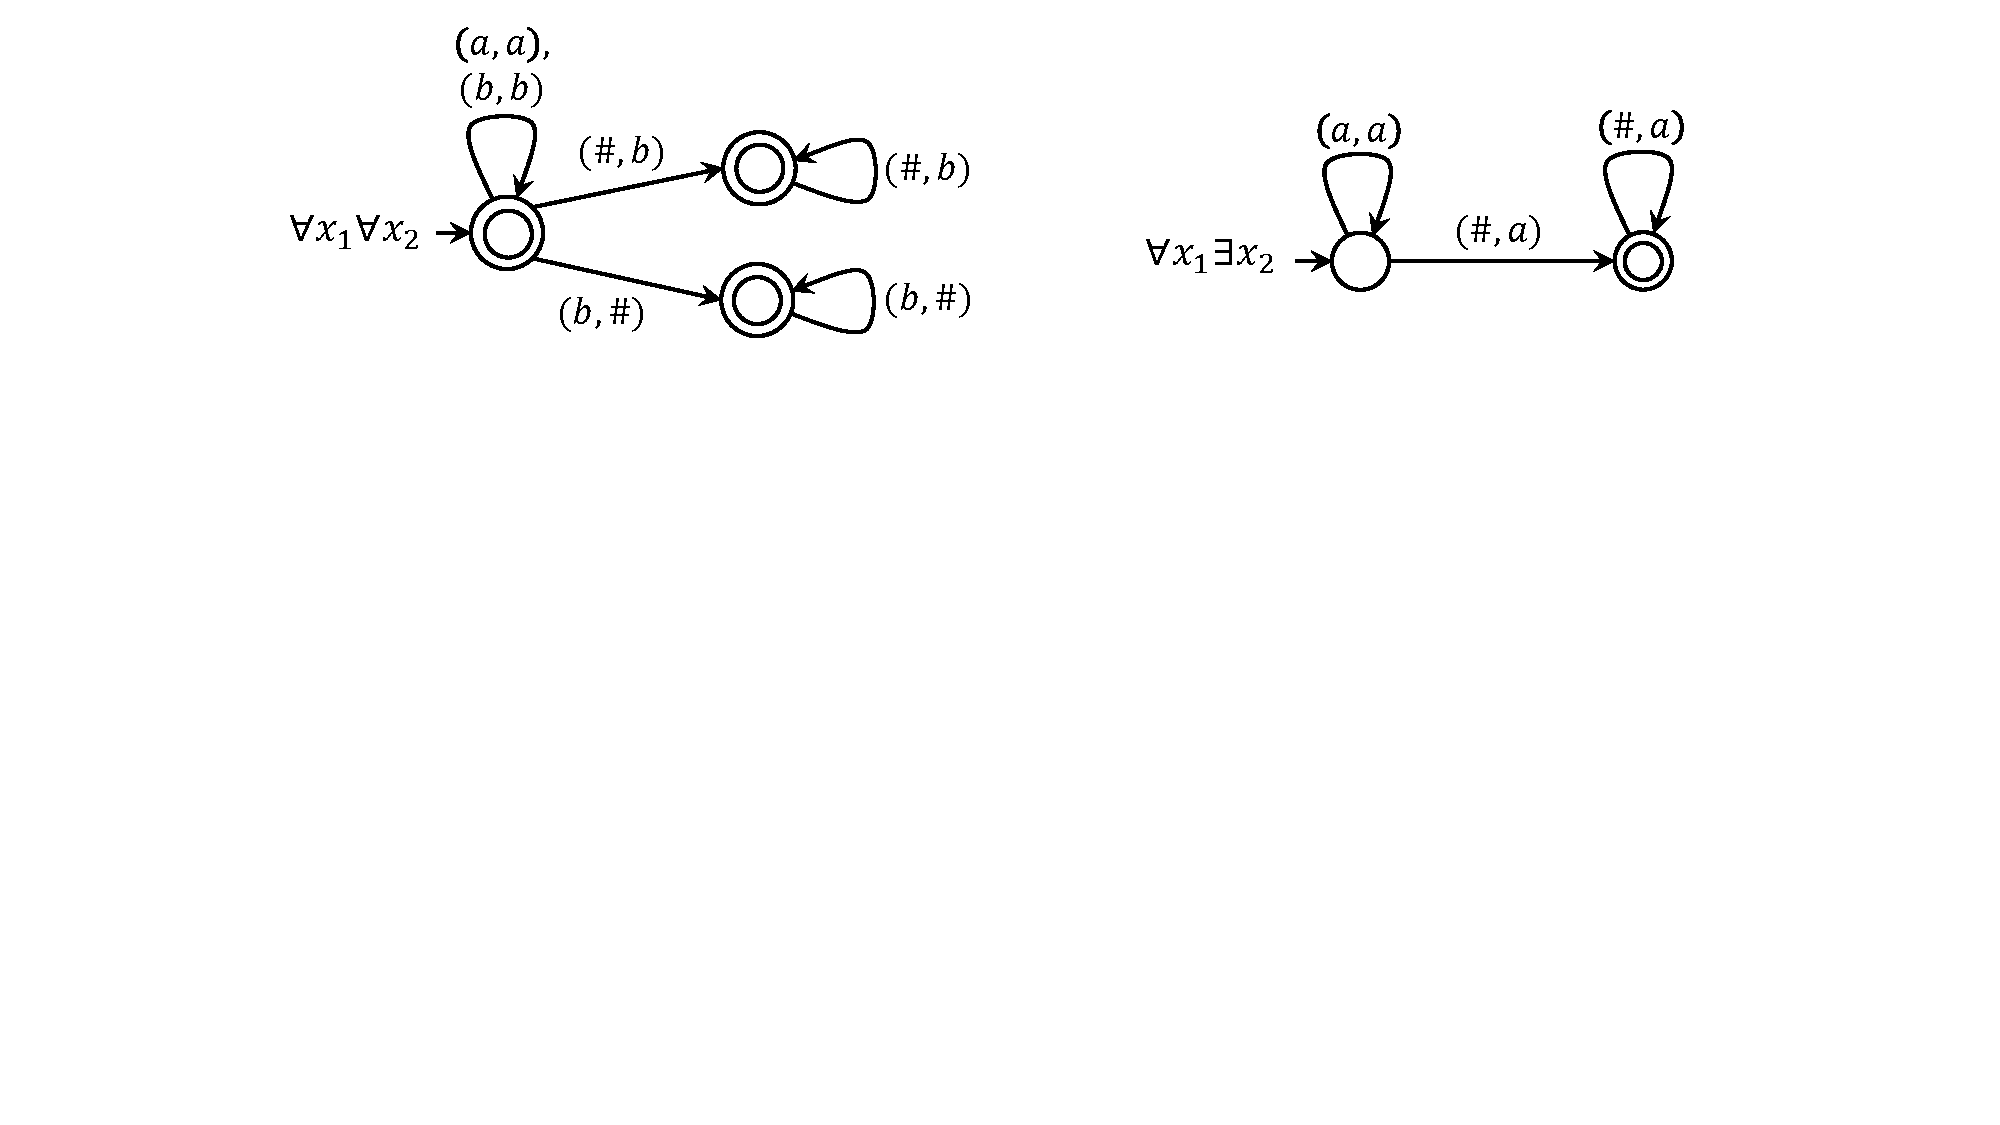
\includegraphics[scale=0.5]{figures/examples.pdf}
    \end{center}
    \caption{The NFH $\A_1$ (left) and $\A_2$ (right).}
    \label{fig:nfh_examples}
%    \hrulefill
\end{figure}


\begin{figure}[ht]
%\hrulefill
    \begin{center}
        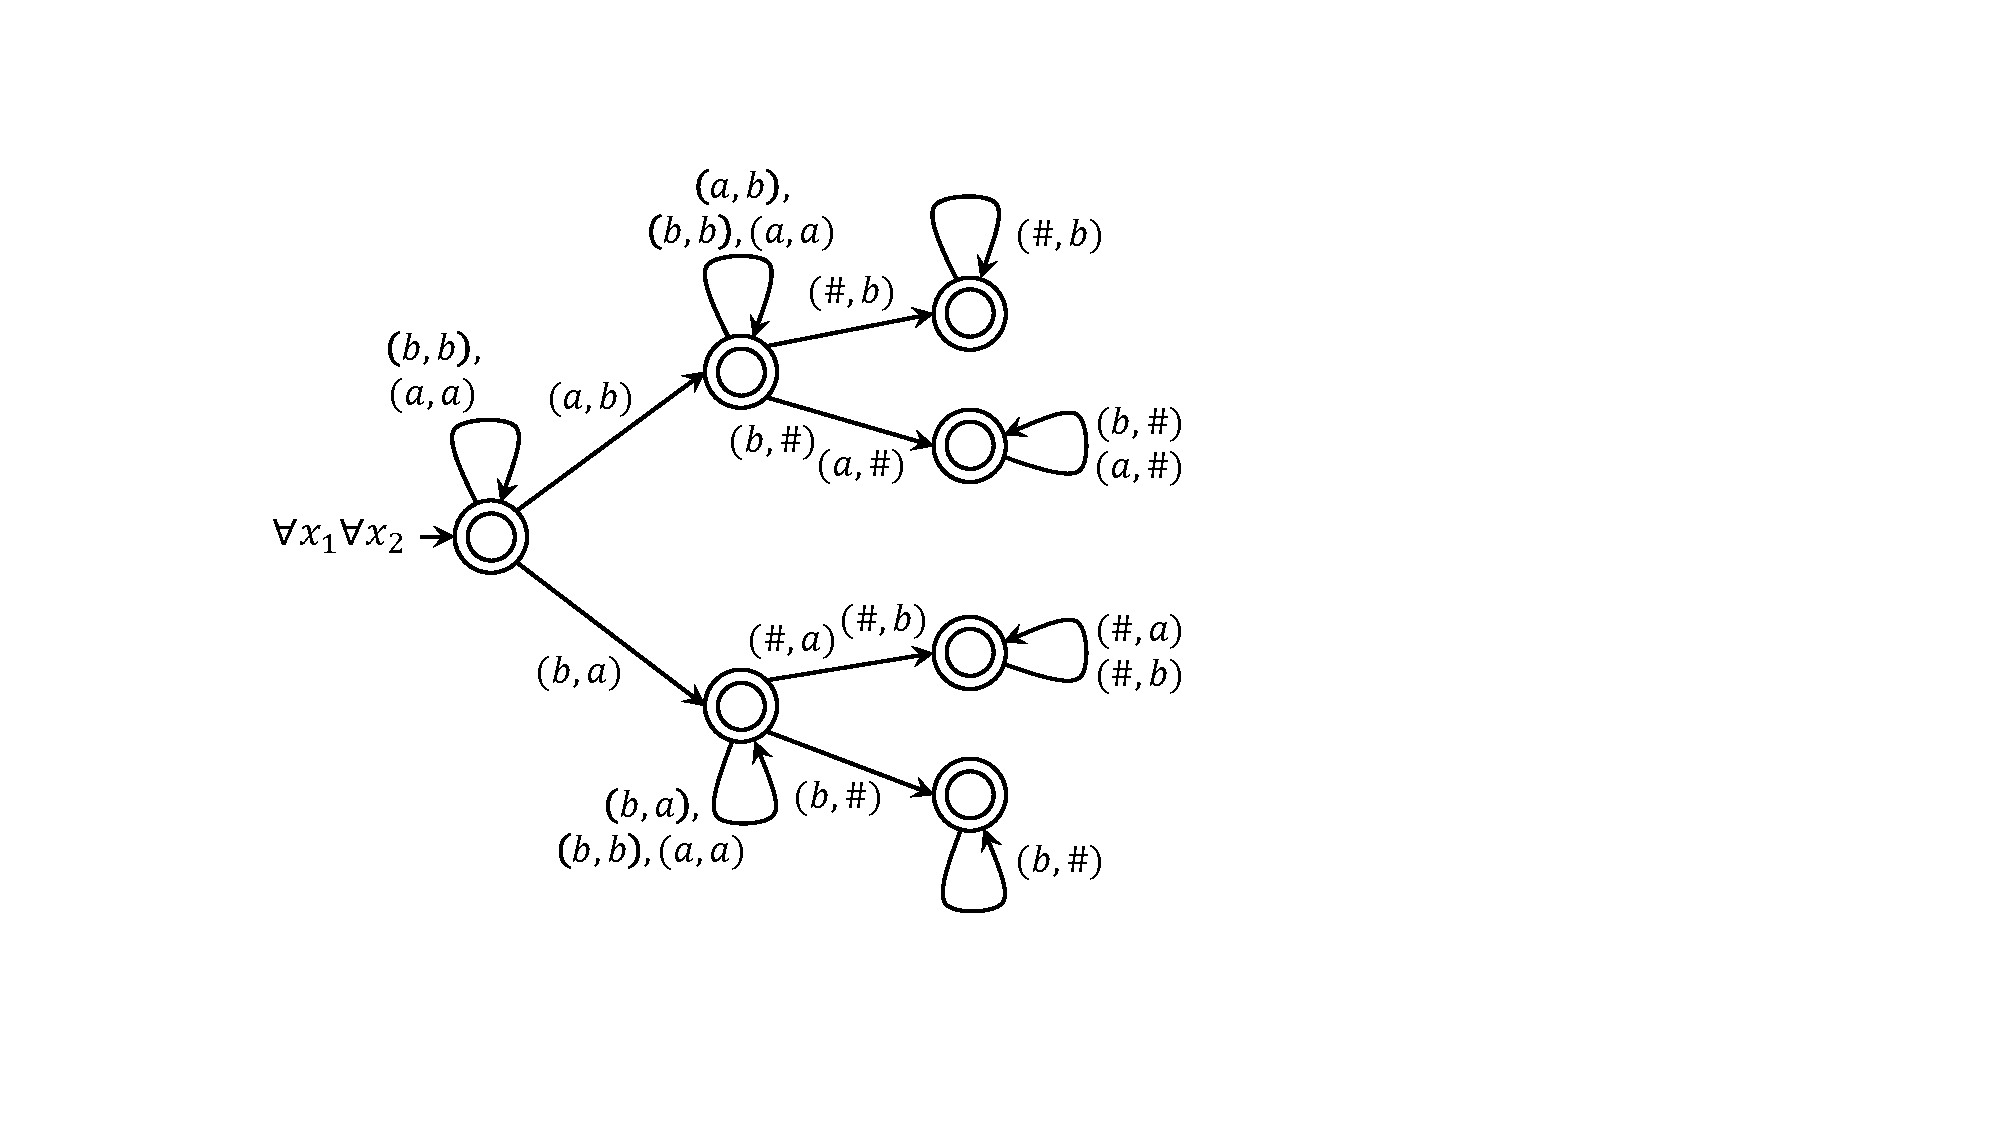
\includegraphics[scale=0.5]{figures/a_implies_a.pdf}
    \end{center}
    \caption{The NFH $\A_3$.}
    \label{fig:ordered}
%    \hrulefill
\end{figure}
\end{example}



We consider several fragments of NFH, which limit the structure of the quantification condition $\alpha$.
$\nfhf$ is the fragment in which $\alpha$ contains only $\forall$ quantifiers, 
and similarly, in $\nfhe$, $\alpha$ contains only $\exists$ quantifiers. In 
$\nfhef$ $\alpha$ is of the form $\exists x_1 \cdots \exists x_i \forall 
x_{i+1}\cdots \forall x_k$, and finally, in $\nfhfe$, $\alpha$ is of the form  
$\forall x_1 \cdots \forall x_i \exists x_{i+1}\cdots \exists x_k$.





%\subsection{Hyperautomata over Hyper-infinite Words}

We now lift the notion of hyperautomata to infinite words. 
A {\em hyper-infinite word} over $\Sigma$ is a set of infinite words over $\Sigma$. 
As before, an automaton $\A$ for a hyperlanguage $\cal L$ consists of an underlying automaton which runs on the tuples of words that are assigned to the word variables of $\A$. In the case of hyper-infinite words, the underlying automaton runs on tuples of infinite words. We consider a B{\"u}chi acceptance condition for the underlying automata. 

\begin{definition}
A {\em nondeterministic B{\"u}chi hyper-word automaton (NBH)} is a tuple $\A = 
\tuple{\Sigma, X=\{x_1,\ldots x_k\}, Q, Q_0, \delta, F, \alpha}$, where all 
elements are as in NFH and acceptance condition defined by the underlying NBW 
of $\A$ is $\hat{\A} = \tuple{\Sigma^k,Q,Q_0,\delta,F}$.

\end{definition}

In particular, consider a hyper-infinite word $S$ and an 
assignment $v:X\rightarrow S$. Then $\hat\A$ accepts $\zip(v)$ iff the run of 
$\hat\A$ on $\zip(v)$ visits some state in $F$ infinitely often. 
The definition of $\models$, acceptance, and $\lang{A}$ are all as in NFH.
As with NFH, we consider the different fragments of NBH$_\forall$, NBH$_\exists$, NBH$_{\forall\exists}$ and NBH$_{\exists\forall}$.




%\section{Hyper Regular Expressions}
\todo{Sarai: I think that we should drop the definition. We can say: We can represent a hyper-regular language $HL$ as a hyper-regular expression $\alpha r$, where $r$ is a regular expression for $\hat\A$ in an NFH $\A$ for $HL$, whose quantification condition is $\alpha$. I don't think we need more than that for this idea.}
A {\em hyper regular expression} (HRE) defines a hyperlanguage. HREs are 
inductively defined by the following grammar:
%
\todo{Sarai: there should also be $\emptyset$ in $\psi$, right?}
\begin{align*}
\varphi ::= & \ \forall x.\varphi \mid \exists x.\varphi \mid \psi\\
\psi ::= & \ \epsilon \mid (a_1, a_2, \ldots a_k) \mid \psi + \psi \mid 
\psi^* \mid \psi\psi
\end{align*}
% 
\todo{Sarai: since we use $k$-tuples, we should probably say that the set of HR is the set of closed (with $k$ quantifiers) expressions. Otherwise the semantics does not make sense.}
where $a_1, a_2, \dots, a_k$ are letters in a finite alphabet $\Sigma$ and $x$ 
is a word variable from an infinite supply $X$.

\todo{Sarai: the syntax and semantics should be separated. Regular expressions are the syntax. For every RE $r$, we assign a hyperlanguage $HL[r]$}The semantics of HREs is as follows. The following constants are 
defined as HREs (obtained by the $\psi$ rule): (1) the empty set $\emptyset$, 
(2) $\{\epsilon\}$ is an HRE, where $\epsilon$ is the empty word, and (3) a 
$k$-tuple of letters $(a_1, a_2, \ldots, a_k)$ is an HRE.
%
Furthermore, HREs can be obtained by the $\psi$ formulas as 
follows: 

\begin{itemize}
\item {\em Concatenation.} \ Let $R_1$ and $R_2$ be two sets of hyperwords. 
$R_1R_2$ denotes the set of hyperwords obtained by concatenating a hyperword in 
$R_1$ and a hyperword in $R_2$. We use the same padding technique for words 
with unequal lengths as described in Section~\ref{sec:ha}. Thus,
%
$$
R_1R_2 = \zip \Big(\unzip(R_1)\cdot\unzip(R_2)\Big)
$$
%
where `$\cdot$' denotes the the standard concatenation operator in regular 
expressions.
For example, let $R_1 
= \{(a, b, c)\}$, and $R_2 = \{(e_1, f_1)(\#, f_2)\}$. Then, 
$R_1R_2 = \{(a, a, b, b, c, c)(e_1, f_1, e_1, f_1)(\#, f_2, \#, 
f_2, \#, f_2)\}$.\todo{Sarai: I don't understand... why is this the concatenation?}

\item {\em Union.} \ $R_1 + R_2$ denotes the set union of sets described 
by $R_1$ and $R_2$:
%
$$
R_1 + R_2 = \zip\Big(\unzip(R_1) \, \cup \unzip(R_2)\Big)
$$
%
For example, if $R_1 = \{(a_1, b_1, a_2, b_2)\}$, and $R_2 
= \{(e_1, f_1)(e_2, f_2)\}$, expression $R_1 + R_2 = 
\{(a_1,b_1, a_2, b_2), (e_1, f_1 \#, \#)(e_2, f_2 \#, \#)\}$.

\item {\em Kleene star.} \ $R^*$ denotes the smallest superset of the set 
described by $R$ that contains $\epsilon$ and is closed under concatenation. 
This is the set of all hyperwords that can be made by concatenating any finite 
number (including zero) of hyperwords from the set described by $R$. For 
example, $((a, a) + (\bar{a}, \bar{a}))^*$, where $\bar{a} \in \Sigma - 
\{a\}$, is the hyperlanguage in which every pair of words agree on the 
position of letter $a$.

\end{itemize}
%
Finally, if $R$ is an HRE obtained by concatenation, alternation, and Kleen 
star only, then $\quant_1x_1.\quant_2x_2.\ldots 
\quant_nx_n R$, where $\quant_i \in \{\forall, \exists\}$, for all $i \in [1, 
n]$ is also an HRE. The semantics of quantified $\varphi$ formulas is the same 
as NHF described in Section~\ref{sec:haf}. 

\begin{theorem}

There is a direct one-to-one correspondence between the grammar of HRE and 
NHF, such that the grammar generates exactly the language the automaton accepts.

\end{theorem}

\begin{proof}
The construction is the same as the standard construction of an NFA from 
a regular expression. The quantification condition $\alpha$ of the NHF will be 
identical to the quantifiers of the input HRE. 
\end{proof}



% We clarify that an HRE cannot be obtained by (1) concatenating two quantified 
% expressions, and (2) applying Kleene star over a quantified expression. Also, 
% union should not created nested quantification.
%\subsection{Semantics of NFH}
% We now formally describe the semantics of NFH, and begin with some terms and 
% notations.


% The semantics of quantification is as follows. As we have noted, a hyperword 
% over $\Sigma$ is $S\subseteq \Sigma^*$. Let $X=\{x_1,\dots, x_k\}$ is a finite 
% set of {\em word variables} be a set of {\em word variables} and $v: 
% X\rightarrow S$ be an assignment of the word variables to words in $S$.
% We represent $v$ by the word $\zip(v) = \bi{v} = \zip(v(x_1),\ldots v(x_k))$.  
% 
% We now define the acceptance condition of a hyperword $S$ by an NFH $\A$. We 
% first define the satisfaction relation $\models$ for a hyperword $S$, an NFH 
% $\A$ over the set of variables $X = \{x_1,\ldots x_k\}$, a quantification 
% condition $\alpha$, and an assignment $v:X\rightarrow S$.
% 
% \begin{itemize}
%     \item For $\alpha = \epsilon$, we denote $S \models _v (\alpha,\A)$ iff 
% $\hat\A$ accepts $\zip(v)$. 
% 
% \item For $\alpha = \exists x_i \alpha'$, we denote $S\models_v \alpha,\A$ iff 
% there exists $w\in S$ such that $S \models_{v[x_i\rightarrow w]}  \alpha',\A$.
% 
% \item For $\alpha = \forall x_i \alpha'$, we denote $S\models_v \alpha',\A$ iff 
% for every $w\in S$, it holds that $S \models_{v[x_i\rightarrow w]}  \A$.
% 
% \end{itemize}
% When $\alpha$ includes all of $X$, then the satisfaction is independent of the 
% assignment $v$, and we denote $S \models \A$, in which case, we say that $\A$ 
% accepts $S$.




\section{Hyper Regular Expressions and Application in Security}

It is straightforward to see that the underlying NFM of an NHF defines a 
regular expression over hyperwords. Such a regular expression along with the 
quantification of the NHF constitutes a {\em hyper regular expression} 
(HRE). For example, consider the left NHF $\A_1$. The HRE of this NHF is the 
following:
%
$$
\forall x_1\forall x_2\Big((a, a) \mid (b, b)\Big)^*\Big((\#, b)^* \mid (b, 
\#)^* \Big)
$$
%
We now show the application of HREs in specifying information-flow 
security policies.

{\em Noninteference}~\cite{gm82} requires that commands issued by users holding 
high clearances be removable without affecting observations of users holding 
low clearances:
%
$$
\varphi_{\mathsf{ni}} = \forall x_1.\exists x_2.(l, l\lambda)^*
$$
%
where $l$ denotes a low state and $l\lambda$ denotes a low state where all high 
commands are replaced by a dummy value $\lambda$.

{\em Observational determinism}~\cite{zm03} requires that if two executions of 
a system start in low-equivalent states, then these execution should remain low 
equivalent:
%
$$
\varphi_{\mathsf{od}} = \forall x_1.\forall x_2. (l, l)^+ + (\bar{l}, 
\bar{l})(\$, \$)^* + (l, \bar{l})(\$, \$)^* + (\bar{l}, l)(\$, \$)^*
$$
%
where $l$ denotes a low state, $\bar{l} \in \Sigma - \{l\}$, and $\$ \in 
\Sigma$. We note that similar polices such as {\em Boudol and Castellani’s 
noninterference}~\cite{bd02} can be formulated in the same 
fashion\footnote{This policy states that any two executions that start from 
bisimilar states (in terms of memory low-observability, should remain 
bisimilarly low-observable.}.

{\em Generalized noninterference} (GNI)~\cite{m88} allows nondeterminism in 
the low-observable behavior, but requires that low-security outputs may 
not be altered by the injection of high-security inputs:
%
$$
\varphi_{\mathsf{gni}} = \forall x_1.\forall x_2.\exists x_3. \bigg((h, l, hl) 
+ (\bar{h}, l, \bar{h}l) + (h, \bar{l}, h\bar{l}) + (\bar{h}, \bar{l}, 
\bar{h}\bar{l}) \bigg)^*
$$
%
where $h$ denotes the high input, $l$ denotes the low output, $\bar{l} \in 
\Sigma -\{l\}$, and $\bar{h} \in \Sigma - \{h\}$.

{\em Declassification}~\cite{ss00} relaxes noninterference by allowing leaking 
information when necessary. Some programs need to reveal secret information to 
fulfill functional requirements. For example, a password checker must reveal 
whether the entered password is correct or not:
%
$$
\varphi_{\mathsf{dc}} = \forall x_1.\forall x_2. (li,li)(pw, pw)(lo, lo)^+
$$
%
where $li$ denotes low-input state, $pw$ denotes that the password is correct, 
and $lo$ denotes low-output states. We note that for brevity, in the above 
formula, we do not include behaviors where the first two events are not low or 
in the second event, the password in not valid. 

{\em Termination-sensitive noninterference} requires that for two executions 
that
 start from low-observable states, information leaks are not permitted by 
the program's termination behavior:
%
$$
\varphi_{\mathsf{tsni}} = \forall x_1.\forall x_2. (l, l)(\$, \$)^*(l, l)  + 
(\bar{l}, \bar{l})(\$, \$)^* + (l, \bar{l})(\$, \$)^* + (\bar{l}, l)(\$, \$)^*
$$
where $l$ denotes a low state and $\$ \in \Sigma$.


%\section{HyperLTL to HyperABA}

\todo{BB: I think we should clearly define HyperLTL and ABA if we want to keep 
this section. I also think this construction appears in 
https://www.react.uni-saarland.de/publications/FRS15.pdf.}\todo{Sarai: I agree about the definitions. About this construction, it's a little different since there the construction is directly for the purpose of model checking and has the system "built in", so there is no quantification of the automaton, it's a standard word automaton. But indeed the idea is similar. Perhaps we should minimize this section and mention that an extension to infinite words allows a direct translation of hyperltl to hyperautomata}

Let $AP$ be a set of atomic propositions, and let $\g = \quant_1 x_1 \ldots \quant_k x_k \f$ be a hyper-LTL formula. 
We construct a hyper-ABA $\A_\g$ over $(2^{AP})^k$ that accepts a hyperword $S$ iff $S\models\f$. Our construction is directly based on Vardi and Wolper's construction for LTL. 
The set of states $S$ is $sub(\f)$, the set of sub-formulas of $\f$, the initial state is $\f$, the set of accepting states are all subformulas of the type $\neg \f_1\until\f_2$.
To define the transition relation $\delta$, 
we first define the {\em dual} formula $\overline{\alpha}$ for a formula $\alpha$, as follows. Let $\alpha_1,\alpha_2$ be formulas over $S$. 
\begin{itemize}
    \item $\overline{\true} = \false$ and $\overline{\false}=\true$.
    \item $\overline{\alpha} = \neg\overline{\alpha}$, for $\alpha\in S$.
    \item $\overline{\alpha_1\wedge\alpha_2} = \overline{\alpha_1}\vee\overline{\alpha_2}$.
    \item $\overline{\alpha_1\vee \alpha_2} = \overline{\alpha_1}\wedge\overline{\alpha_2}$.
    \item

\end{itemize}

The transition relation $\delta$ is as follows. 
\begin{itemize}
\item $\delta(a_{x_i},\sigma) = \true$ if $a\in\sigma[i]$, and $\false$ otherwise. 
\item $\delta(\nextt \f_1, \sigma) =  \f_1$.
\item $\delta(\f_1\vee \f_2,\sigma) = \delta(\f_1,\sigma)\vee \delta(\f_2,\sigma)$.
\item $\delta(\neg \f_1) = \overline{\delta(\f_1)}$.
\item $\delta(\f_1 \until \f_2, \sigma) = \delta(\f_2,\sigma)\vee (\delta(\f_1,\sigma) \wedge (\f_1\until\f_2))$. 
\end{itemize}

Finally, the quantification condition of $\A_\g$ is $\quant_1 x_1 \ldots \quant_k x_k$. 
\section{Properties of Hyperautomata and Hyper Regular Expressions}
\label{sec:nfh_properties}

%\subsection{Properties of NFH}

In this section, we consider the basic operations and decision problems for the various fragments of NFH. 
Throughout  section, we assume an NFH $\A = \tuple{\Sigma,X,Q,Q_0,\delta,F,\alpha}$ where $X = \{x_1,\ldots x_n\}$. 

%For the various complexity results, notice that  the number of variables $k$ and the number of letters $\Sigma$ dictate an alphabet size of $O(|\Sigma|^k)$ for $\hat\A$. Thus, though the state space of $\hat\A$ is of size $n$, its size may be exponential in the number of variables due to its transition relation, which may be of size $n\times |\Sigma|^k\times n$. 

\begin{theorem} \label{thm:nfh.complement}
NFH are closed under complementation.
\end{theorem}

\begin{proof}
Let $\A$ be an NFH. The NFA $\hat \A$ 
can be complemented with respect to its language over $\hat\Sigma$ to an NFA $\overline{\hat{\A}}$. 
Then, for every assignment $v:X\rightarrow S$, it holds that $\hat \A$ accepts 
$\zip(v)$ iff $\overline{\hat{\A}}$ does not accept $\zip(v)$.

Let $\overline{\alpha}$ be the quantification condition obtained from $\alpha$ by 
replacing every $\exists$ with $\forall$ and vice versa. 
Then, we can prove by induction on $\alpha$, that $\overline{\A}$, the NFH whose 
underlying automaton is $\overline{\hat{\A}}$, and whose quantification condition is 
$\overline{\alpha}$, accepts $\overline {\hlang{\A}}$.

The size of $\overline{\A}$ is exponential in $n$, due to the complementation construction for $\hat\A$.
\qed
\end{proof}


\begin{theorem} \label{thm:nfh.union}
NFH are closed under union.
\end{theorem}

\begin{proof}
The proof is similar to the standard constructive proof for NFAs. Let $\A = 
\tuple{\Sigma,X,Q,Q_0,\delta,F,\alpha}$ with underlying NFA and $\A'= 
\tuple{\Sigma',X',Q',Q'_0,\delta',F',\alpha'}$ be two NHFs. We now construct an 
NHF $\A'' = \tuple{\Sigma'',X'',Q'',Q''_0,\delta'',F'',\alpha''}$ that accepts 
$\hlang{\A} \cup \hlang{\A'}$ as follows. Let
%
\begin{itemize}
 \item  $\Sigma'' = \Sigma \cup \Sigma' \cup \{\#\}$,
 \item $X'' = X \cup X'$,
 \item $Q'' = Q \cup Q' \cup \{q_{\mathit{init}}\}$, \todo{Sarai: we allow a set of inital state, so taking the union is enough, no need for a new state}
 \item $Q''_0 = q_{\mathit{init}}$,
 \item $F'' = F \cup F'$,
 \item $\alpha'' = \alpha.\alpha'$
 
\end{itemize}
%
Transitions of $\A''$ include the following:

\begin{itemize}
 \item  We add transitions $q\xrightarrow{\epsilon} q'$, for each $q' \in 
Q''_0$, where $\epsilon$ is the null letter. 

\item For each transition $q \xrightarrow{(\sigma_{i_1}, \dots, \sigma_{i_k})} 
q' \in \delta$ (in the underlying NFA of $\A$), we include a transition $q 
\xrightarrow{(\sigma_{i_1}, \dots, \sigma_{i_k}, \#, \dots, \#)} q'$ in 
$\delta''$, where $\#$ is repeated $|\alpha'|$ number of times (i.e., the number 
of quantifiers in $\alpha$). Likewise, for each transition $q 
\xrightarrow{(\sigma_{i_1}, \dots, \sigma_{i_{k'}})} q' \in \delta'$ (in the 
underlying NFA of $\A'$), we include a transition $q \xrightarrow{(\#, \dots, 
\#, \sigma_{i_1}, \dots, \sigma_{i_{k'}})} q'$ in $\delta''$, where $\#$ is 
repeated $|\alpha|$ number of times (the number of quantifiers in $\alpha$).
\todo{Sarai: I think this is incorrect. We should not add $\#$, but every possible combination of $\Sigma\cup\{\#\}$ letters}
\end{itemize}

Now, it is straightforward to see that every hyperword in $\hlang{\A}$ or 
$\hlang{\A'}$ is accepted by $\A''$. This is because the quantifiers not 
relevant to hyperwords (e.g., $\alpha$) for a hyperword in $\hlang{\A'}$ are 
taken care of by the padded words in $(\#, \dots, \#, \sigma_{i_1}, \dots, 
\sigma_{i_{k'}})$. The same argument holds for quantifiers in $\alpha'$ and 
hyperwords in $\hlang{\A}$.\qed

\end{proof}


\begin{theorem}\label{thm:nfh.intersection}
NFH are closed under intersection.
\end{theorem}

\begin{proof}
The proof follows the closure under union and complementation. However, we can also offer a direct translation, which avoids the need to complement. 
Given two NFH $\A_1 = 
\tuple{\Sigma,X,Q,Q_0,\delta_1,F_1,\alpha_1}$ and $\A_2= 
\tuple{\Sigma,Y,P,P_0,\delta_2,F_2,\alpha_2}$, we construct an NFH $\tuple{\Sigma,X\cup Y, (Q\cup \{q\} \times P\cup \{p\}, P_0\times Q_0, \delta, (F_1\cup\{q\}) \times (F_2\cup\{p\}), \alpha}$, where 
$\alpha = \alpha_1\alpha_2$, and $\delta$ is defined as follows. 
\begin{itemize}
    \item For every $(q_1\xrightarrow {(\sigma_1,\ldots \sigma_k)} q_2)\in \delta_1$ and every $(p_1\xrightarrow {(\sigma'_1\ldots \sigma'_{k'}) }p_2)\in\delta_2$, we have 
$$((q_1,p_1)\xrightarrow{(\sigma_1\ldots \sigma_k,\sigma'_1,\ldots \sigma'_{k'})} (q_2,p_2))\in\delta$$
\item For every $q_1\in F_1, (p_1 \xrightarrow{(\sigma'_1,\ldots \sigma'_{k'})} p_2)\in \delta_2$ we have $$((q_1,p_1)\xrightarrow {(\overbrace{\#,\ldots\#}^{k},\sigma'_1,\ldots \sigma'_{k'})}(q,p_2)), ((q,p_1)\xrightarrow {(\overbrace{\#,\ldots\#}^{k},\sigma'_1,\ldots \sigma'_{k'})}(q,p_2)) \in \delta$$
\item For every $(q_1\xrightarrow {(\sigma_1,\ldots \sigma_k)} q_2)\in \delta_1$ and $p_1\in F_2$, we have $$((q_1,p_1)\xrightarrow {(\sigma_1,\ldots \sigma_{k},\overbrace{\#,\ldots\#}^{k'})}(q_2,p)),((q_1,p)\xrightarrow {(\sigma_1,\ldots \sigma'_{k},\overbrace{\#,\ldots\#}^{k'})}(q_2,p))\in \delta$$
\end{itemize}

Intuitively, the role of $q,p$ is to keep reading $(\#)^k$ and $(\#)^{k'}$ after the word read by $\hat\A_1$ or $\hat\A_2$, respectively, has ended. 

The NFH $\hat\A$ simultaneously reads two words $\zip(w_1,\ldots w_k)$ and $\zip(w'_1,w'_2,\ldots w'_{k'})$ that are read along $\hat\A_1$ and $\hat\A_2$, respectively, and accepts only if both words are accepted. The correctness follows from the fact that for $v:(X\cup Y)\rightarrow S$, we have that $\zip(v)$ is accepted by $\hat\A$ iff $\zip (v|_X)$ and $\zip(v|_Y)$ are accepted by $\hat\A_1$ and $\hat\A_2$, respectively. 

This construction is polynomial in the sizes of $\A_1$ and $\A_2$.
\end{proof}


We now turn to study various decision problems for NFH. We begin with the nonemptiness problem: given an NFH $\A$, is $\hlang{\A} = \emptyset$? We show that while the problem is in general undecidable for NFH, it is decidable for most fragments that we consider. 


\begin{theorem}
The nonemptiness problem for NHF is undecidable.
\end{theorem}

\begin{proof}

We mimic the proof in \cite{fh16}, with a reduction from the {\em post correspondence problem (PCP)}.
%
The PCP is as follows.
%
Fix an alphabet $\alphabet_{\mathit{pcp}}$ of size at least two. \todo{Sarai: we can just use $a,b$}
%
Given is a collection of dominos of the form:
$$\Big[\frac{w}{v} \Big] = \bigg\{\Big[\frac{w_1}{v_1} \Big], 
\Big[\frac{w_2}{v_2} \Big],\dots, \Big[\frac{w_k}{v_k} \Big] \bigg\}$$
where for all $i \in [1, k]$, we have $v_i,w_i \in \alphabet_{\mathit{pcp}}^*$.
%
The decision problem consists of whether there exists a finite sequence of
dominos of the form
$$\Big[\frac{w_{i_1}}{v_{i_1}} \Big]\Big[\frac{w_{i_2}}{v_{i_2}} \Big] \cdots 
\Big[\frac{w_{i_m}}{v_{i_m}} \Big]$$
where each index $i_j \in [1, k]$, such that the upper and lower finite strings 
of the dominos are equal, i.e.,
$$v_{i_1}v_{i_2}\cdots{}v_{i_m} = w_{i_1}w_{i_2}\cdots{}w_{i_m}.$$
%
For some collection of dominos, it is impossible to find a match. An example is 
the following:
$$\Big[\frac{w}{v} \Big] = \bigg\{\Big[\frac{abc}{ab} \Big], \Big[\frac{ca}{a} 
\Big], \Big[\frac{acc}{ba} \Big]\bigg\}$$

\stam{
First, we map an arbitrary instance of the PCP 
$[\frac{w}{v}]=\{[\frac{w_2}{v_2}], [\frac{w_2}{v_2}], \dots, 
[\frac{w_k}{v_k}]\}$ to an NHF.
}

Given an instance $C$ of PCP, we encode a solution as a word $w_{sol}$ over $\alphabet = \{\frac{\sigma}{\sigma'}| \sigma,\sigma'\in\{a,b,{\dot a},{\dot b}, \$\}\}$.

For a word $w = \frac{\sigma_1}{\sigma'_1}   \frac{\sigma_2}{\sigma'_2}  \cdots  \frac{\sigma_n}{\sigma'_n}  $, we call $\sigma_1\cdots \sigma_n$ the {\em upper part} of $w$, and the word $\sigma'_1\cdots \sigma'_n$ the {\em lower part} of $w$. 

Intuitively, $\dot{\sigma}$ marks the beginning of a new tile, and $\$$ marks the end of a sequence of the upper or lower parts of the dominos.

$w_{sol}$ encodes a legal solution if the following conditions are met.
\begin{enumerate}
    \item For every $ \frac{\sigma}{\sigma'}  $ that occurs in $w_{sol}$, it holds that $\sigma,\sigma'$ represent the same domino letter (both $a$ or both $b$).
    \item and the number of dotted letters in the upper part of $w_{sol}$ is equal to the number of dotted letters in the lower part of $w_{sol}$.
    \item $w_{sol}$ starts with two dotted letters, and the word $u_i$ between the $i$'th and $i+1$'th dotted letters in the upper part of $w_{sol}$, and the word $v_i$ between the corresponding dotted letters in the lower part of $w_{sol}$ are such that $ \frac{u_i}{v_i}  \in C$.
\end{enumerate}

%A {\em partial solution} is a word $w\in \Sigma^*$ that only satisfies conditions $2$ and $3$, and in which $\$$ does not occur in either part (lower or upper) before an $a$ or $b$ representation in this part.
We call a word that represents the removal of the first $k$ tiles from $w_{sol}$ a {\em partial solution}, denoted by $w_{sol,k}$.
Note that the upper and lower parts of $w_{sol,k}$ are not necessarily of equal lengths (in terms of $a$ and $b$ sequences), since the upper and lower parts of a domino tile are not necessarily of equal lengths, and so $\$$ is used to pad the end of the encoding in the shorter of the parts. 

We construct an NFH $\A$, which, intuitively, expresses the following idea: $(1)$ there exists an encoded solution $w_{sol}$, and $(2)$ For every $w_{sol,k}$ in a hyperset $S$ accepted by $\A$, the word $w_{sol,k+1}$ is also in $S$. 

$\hlang{\A}$ is then the set of all hyperwords that consist of a solution $w_{sol}$, and all its suffixes obtained by removing a prefix of tiles from $w_{sol}$.  

For example, if the set of tiles is 
$$ \{ [\frac{ab}{b}], [\frac{ba}{a}],[\frac{a}{aba}] \} $$
Then a possible solution is 
$$ [\frac{a}{aba}][\frac{ba}{a}] [\frac{ab}{b} ]  $$
and so a matching hyperword $S$ that is accepted by $\A$ is
$$ S = \{  w_{sol} = \frac{\dot a}{\dot a}   \frac{\dot b}{b}   \frac{a}{a}   \frac{\dot a}{\dot a}   \frac{b}{\dot b} ,
w_{sol,1} = \frac{\dot b}{\dot a}\frac{a}{\dot b}\frac{\dot a}{\$}\frac{b}{\$}, w_{sol,2} = \frac{\dot a}{\dot b}\frac{b}{\$}, w_{sol,3} = \epsilon
\} $$

Thus, the acceptance condition of $\A$ is $\alpha = \forall x_1\exists x_2 \exists x_3$, where $x_1$ is to be assigned a partial solution $w_{sol,k}$, the variable $x_2$ is to be assigned $w_{sol,k+1}$, and $x_3$ is to be assigned $w_{sol}$.  

During a run on a hyperword $S$ and an assignment $v:\{x_1,x_2,x_3\}\rightarrow S$, the NFH $\A$ checks that the upper and lower letters of $w_{sol}$ all match.
In addition, it checks that $v(x_2)$ is obtained from $v(x_1)$ by removing the first tile. 

It does so by remembering, using the states, the  




\todo{TBC}
\end{proof}



\begin{theorem} \label{thm:nfhe.nfhf.nonemptiness}
The nonemptiness problem for $\nfhe$ and $\nfhf$ is NL-complete.
\end{theorem}

\begin{proof}
We begin with $\nfhe$. Let $\A_\exists$ be an $\nfhe$ over a set of variables $X 
= \{x_1,x_2,\ldots x_k\}$. 
Let $w$ be a word over $(\Sigma\cup \#)^k$. We say that $w$ is {\em legal} if 
$w=\zip(u_1,\ldots u_k)$ for $u_1,u_2,\ldots u_k \in \Sigma^*$. 
Note that $w$ is legal if there is no $w[i]$ in which there is a $\#$ that is 
followed by some $\sigma\in \Sigma$. 
We claim that $\A_\exists$ is nonempty iff $\hat\A_\exists$ accepts some legal 
word $w$. The first direction is trivial. For the second direction, let 
$w\in\lang{\hat\A_\exists}$, and let $S$ be the set of words in $\unzip(w)$. By 
assigning $v(x_i) = w[i]$ for every $x_i\in X$, we get $\zip(v) = w$, and 
according to the semantics of $\exists$, we have that $\A_\exists$ accepts $S$. 
To check whether $\hat\A_\exists$ accepts a legal word, we can run a 
reachability check on-the-fly, while advancing from a letter $\sigma$ to the 
next letter $\sigma'$ only if $\sigma'$ contains $\#$ in all the positions in 
which $\sigma$ contains $\#$. 
While each transition $T = q\xrightarrow{(\sigma_1,\ldots \sigma_n)} p$ in $\hat\A$ is of size $k$, we can encode $t$ as a set of size $k$ of encodings of transitions of type $q \xrightarrow {\sigma_i} p$, with a binary encoding of $p,q,\sigma_i$, as well as $i,t$, where $t$ marks the index of $T$ within the set of transitions of $\hat\A$. 
Now, let $\A_\forall$ be an $\nfhf$ over $X$. We claim that $\A_\forall$ is 
nonempty iff $\A_\forall$ accepts a hyperword of size $1$. 
For the first direction, let $S\in\lang{\A_\forall}$. Then, by the semantics of 
$\forall$, we have that for every assignment $v:X\rightarrow S$, it holds that 
$\zip(v)\in\hat{\A_\forall}$. Let $u\in S$, and let $v_u(x_i) = u$ for every 
$x_i\in X$. Then, in particular, $\zip(v_u)\in\lang{\hat{\A_\forall}}$. We have 
then that for every assignment $v:X\rightarrow \{u\}$ (which consists of the 
single assignment $u_v$), it holds that $\hat{\A_\forall}$ accepts $\zip(v)$, 
and therefore $\A_\forall$ accepts $\{u\}$. 
The second direction is trivial. 

To check whether $\A_\forall$ accepts a hyperword of size $1$, we restrict the 
alphabet of $\hat\A_\forall$ to $k$-tuples of the form $(\sigma,\sigma,\ldots 
\sigma)$ for $\sigma\in \Sigma$, by removing all other transitions. Then, we 
check whether the remaining NFA is nonempty. 

Since the nonemptiness problem for NFA is NL-complete, the results for both 
fragments follow. 
\end{proof}

We now show that the nonemptiness problem for $\nfhef$ is decidable. We first 
present some terms and notations.  

Consider a tuple $t = (t_1,t_2,\ldots t_k)$ of items. 
A {\em sequence} of $t$ is a tuple $(t'_1, t'_2,\ldots t'_k)$, where 
$t'_i\in\{t_1,\ldots t_k\}$ for every $1\leq i \leq k$. 
A {\em permutation} of $t$ is a reordering of the elements of $t$. 
We extend the notion of permutation to words over $k$-tuples, and to 
assignments, as follows. 
Let $w = \zip(w_1,\ldots w_k)$ be a word over $k$-tuples, and let $\zeta = 
(i_1,i_2,\ldots i_k)$ be a sequence (permutation) of $(1,2,\ldots, k)$. The word $w_\zeta$, 
defined as $\zip(w_{i_1}, w_{i_2}, \ldots w_{i_k})$ is a sequence (permutation) of $w$.
Finally, let $v$ be an assignment from a set of variables $\{x_1,x_2,\ldots 
x_k\}$ to a hyperword $S$. The assignment $v_\zeta$, defined as $v_\zeta(x_j) = 
v(x_{i_j})$ for every $1\leq i,j \leq k$, is a sequence (permutation) of $v$. 
\todo{Sarai: move this elsewhere? since we use these terms also in learning}

We now show that if an $\nfhef$ is nonempty, then we can bound the size of a 
hyperword that it accepts.

\begin{lemma}\label{lemma:nfhef.nonempty}
Let $\A$ be an $\nfhef$ with a quantification condition $\alpha = \exists x_1,\ldots \exists x_m \forall 
x_{m+1}\ldots \forall x_k$, where $1 \leq m < k$. 
Then $\A$ is nonempty iff $\A$ accepts a hyperword of size at most $m$.
\end{lemma}

\begin{proof}
Let $S\in\hlang{\A}$. Then according to the semantics of the quantifiers, there 
exist $w_1,\ldots w_m \in S$, such that for every 
assignment $v:X\rightarrow S$ in which $v(x_i) = w_i$ for every $1\leq i\leq m$, 
it holds that $\hat\A$ accepts $\zip(v)$.
Let $v:X\rightarrow S$ be such an assignment.
Then $\hat\A$ accepts 
$\zip(v_\zeta)$ for every sequence $\zeta$ of the form $(1,2,\ldots m,i_1,i_2,\ldots 
i_{m-k})$. 
In particular, it holds for such sequences in which 
$1\leq i_j\leq m$ for every $1\leq j \leq k-m$,
that is, sequences in which the last $k-m$ variables are assigned words from 
the set of words that are assigned to the first $m$ variables. Therefore, again 
by the semantics of the quantifiers, we have that $\{v(x_1),\ldots v(x_m)\}$ is 
in $\hlang{\A}$.
The second direction is trivial.
\end{proof}

We now use Lemma~\ref{lemma:nfhef.nonempty} to describe a decision procedure for 
the nonemptiness of $\nfhef$. 

\begin{theorem}\label{thm:nfhef.nonemptiness}
The nonemptiness problem for an $\nfhef$ $\A$ can be decided in space that is polynomial in the size of $\hat\A$.
\end{theorem}

\begin{proof}
Let $\A$ be as described in Lemma~\ref{lemma:nfhef.nonempty}.
According to Lemma~\ref{lemma:nfhef.nonempty}, 
$\A$ is nonempty iff there exists a word $w\in\lang{\hat\A}$ such that
$\hat\A$ accepts $w_\zeta$ for every sequence $\zeta$ of the form $(1,2,\ldots m, 
i_1,i_2,\ldots i_{k-m})$, where $1\leq i_j\leq m$ for every $1\leq j \leq k-m$.
Indeed, by the semantics of the quantifiers, it holds that $\A$ accepts 
$\{w[1],w[2],\ldots w[m]\}$.
We call $w$ a {\em witness to the nonemptiness of $\A$}.

We construct an NFA $A$ based on $\hat\A$ that is nonempty iff $\hat\A$ accepts 
a witness to the nonemptiness of $\A$.
Let $\Gamma$ be the set of all sequences of the above form.
For every sequence $\zeta = (i_1,i_2,\ldots i_k)$ in $\Gamma$, we construct 
an NFA $A_\zeta = \tuple{ \hat\Sigma,Q,Q_0,\delta_\zeta,F}$, where for every 
$q\xrightarrow{(\sigma_{i_1},\sigma_{i_2},\ldots \sigma_{i_k})} q'$ in $\delta$, 
we have $q\xrightarrow{(\sigma_1,\sigma_2,\ldots \sigma_k)} q'$ in 
$\delta_\zeta$.
Intuitively, $A_{\zeta}$ runs on every word $w$ the same way that $\hat\A$ runs 
on $w_\zeta$. Therefore, $\hat\A$ accepts a witness $w$ to the nonemptiness of 
$\A$ iff $w\in\lang{A_\zeta}$ for every $\zeta\in\Gamma$. 

We define $A = \bigcap_{\zeta\in\Gamma} A_\zeta$.
Then $\hat\A$ accepts a witness to the nonemptiness of $\A$ iff $A$ is 
nonempty. 
Since $|\Gamma| = m^{k-m}$, the state space of $A$ is of size $O(n^{m^{k-m}})$, and its alphabet is of size $|\hat\Sigma|$. 

Notice that for $\A$ to be nonempty, $\hat\Sigma$ must be of size at least $|(\Sigma\cup {\#})|^{(k-m)}$, to account for all the permutations of letters in the words assigned to the variables under $\forall$ quantifiers (otherwise, we can immediately return ``empty''). Therefore, $|\hat\A|$ is $O(n\times \Sigma^k)$. 
We then have that the size of $A$ is $O(|\hat \A|^k)$.  

If the number $k-m$ of $\forall$ quantifiers is fixed, then $m^{k-m}$ is polynomial in $k$. However, now $|\hat\A|$ may be polynomial in $n,k,|\Sigma|$, and so in this case as well, the size of $A$ is $O(|\hat A|^k)$. 

Since the nonemptiness problem for NFA is NL-complete, the problem for $\nfhef$ can be solved in space that is polynomial in $|{\hat\A}|$. 

\end{proof}

\begin{theorem}
The nonemptiness problem for $\nfhef$ is  PSPACE-complete.
\end{theorem}
\begin{proof}
The upper bound follows from Theorem~\ref{thm:nfhef.nonemptiness}. 
For the lower bound, we show a reduction from a polynomial version of the {\em tiling problem}, %~\cite{Boas97}, 
defined as follows.
We are given a finite set $T$ of tiles, two relations $V \subseteq T \times T$ and $H \subseteq T \times T$,
an initial tile $t_0$, a final tile $t_f$, and a bound $n>0$.
We have to decide whether there is some $m>0$ and a tiling of a $n \times m$-grid such that
(1) The tile $t_0$ is in the bottom left corner and the tile $t_f$ is in the top right corner,
(2) A horizontal condition: every pair of horizontal neighbors is in $H$, and
(3) A vertical condition: every pair of vertical neighbors is in $V$.

When $n$ is given in unary, the problem is known to be PSPACE-complete.

Given an instance $C$ of the tiling problem, We construct an $\nfhef$ $\A$ that is nonempty iff $C$ has a solution. 
We encode a solution to $C$ as a word $w_{sol} =w_1\cdot w_2\cdot w_m\$$ over $T$, where $w_i$, of the form $1\cdot t_{1,i}\cdot 2 \cdot t_{2,i},\ldots n\cdot t_{n,i}$, describes the contents of row $i$. 

To check that $w_{sol}$ indeed encodes a solution, we need to make sure that:
\begin{enumerate}
\item $w_1$ begins with $t_0$ and $w_m$ ends with $t_f\$$,
\item Within every $w_i$, it holds that $(t_{j,i},t_{j+1,i})\in H$,
    \item $w_i$ is of the correct form,
    \item For $w_i,w_{i+1}$, it holds that $(t_{j,i}, t_{j,i+1})\in V$ for every $1\leq j\leq n$
\end{enumerate} 

Verifying items $1-3$ is easy via an NFA of size $O(n|H|)$.  
The main obstacle is item $4$. 

We describe an $\nfhef$ $\A = \tuple{T\cup \{0,1,2,\ldots n,\$\}, \{y_1,y_2,y_3,x_1,\ldots x_{\log(n)}\}, Q, \{q_0\},\delta, F, \alpha}$ that is nonempty iff there exists a word that satisfies items $1-4$.
The quantification condition $\alpha$ is $\exists y_1\ldots \exists y_3\forall x_1 \ldots \forall x_{\log(n)}$.
$\A$ only proceeds on letters whose first three positions are of the type $(r,0,1)$, where $r\in T\cup\{1,\ldots n,\$\}$. Notice that this means that it requires the existence of the words $0^{|w_{sol}|}$ and $1^{|w_{sol}|}$ (the $0$ word and $1$ word, henceforth).
$\A$ makes sure that the word assigned to $y_1$ matches a correct solution w.r.t. items $1-3$ described above.  
We proceed to describe how to handle the requirement for $V$. 
We need to make sure that for every position $j$ in a row, the tile in position $j$ in the next row matches the current one w.r.t. $V$. We can use a state $q_j$ to remember the tile in position $j$, and compare it to the tile in the next occurrence of $j$. The problem is avoiding having to check all positions simultaneously, which would require exponentially many states. To this end, we use $\log(n)$ copies of the $0$ and $1$ words to form a binary encoding of the position $j$ that is to be remembered. The $\log(n)$ $\forall$ conditions make sure that every position within $1-n$ is checked.  

We limit the checks to words in which $x_1,\ldots x_{\log(n)}$ are the $0$ or $1$ words, by having $\hat\A$ accept every word in which there is a letter that is not over $0,1$ in positions $4,\ldots \log(n)+3$. Notice that this takes care of accepting all cases in which the word assigned to $y_1$ is also assigned to one of the $x$ variables. 

To check that $x_1,\ldots x_{\log(n)}$ are the $0$ or $1$ words, $\hat\A$ checks that the values in positions $4$ to $\log(n)+3$ remain constant throughout the run. 
In these cases, upon reading the first letter, $\hat\A$ remembers the value $j$ that is encoded by the constant assignments to $x_1,\ldots x_{\log(n)}$ in a state, and makes sure that throughout the run, the tile that occurs in the assignment $y_1$ in position $j$ in the current row matches the tile in position $j$ in the next row. 

We can construct a similar reduction for the case that the number of $\forall$ quantifiers is fixed: instead of encoding the position by $\log(n)$ bits, we can directly specify the position by a word of the form $j^*$, for every $1\leq j\leq n$. 
Accordingly, we construct an $\nfhef$ over $\{x, y_1,\ldots y_{n},z\}$, with a quantification condition $\alpha = \exists x\exists y_1 \ldots \exists y_{n}\forall z$. The NFA $\hat\A$ advances only on letters whose assignments to $y_1,\ldots y_n$ are always $1,2,\ldots n$, respectively, and checks only words assigned to $z$ that are some constant $1\leq j\leq n$. Notice that the fixed assignments to the $y$ variables leads to $\hat\Sigma$ of polynomial size.  
In a hyperword accepted by $\A$, the word assigned to $x$ is $w_{sol}$, and the word assigned to $z$ specifies which index should be checked for conforming to $V$.
\end{proof}

We turn to study the membership problem for NFH: given an NFH $\A$ and a hyperword $S$, is $S\in\hlang{\A}$? 
When $S$ is finite, the set of assignments from $X$ to $S$ is finite, and so the problem is decidable. We call this case the {\em finite membership problem}. 

\begin{theorem}\label{thm:nfh.membership.finite}
Let $\A$ be an NFH and $S$ be a finite hyperword over $\Sigma$. Then it can be decided whether $S\in \hlang{\A}$ in space that is polynomial in $k$, and logarithmic in $|\hat\A|, |S|$.
\end{theorem}

\begin{proof}
As discussed in the proof of Theorem~\ref{thm:nfhef.nonemptiness}, the size of $\hat\Sigma$ must be exponential in the number of $\forall$ quantifiers in $\alpha$, and therefore is exponential in $k$. 
We can decide the membership of $S$ in $\hlang{\A}$ by iterating over all assignments of the type $X\rightarrow S$. For every such assignment $v$, we construct $\zip(v)$ and run $\hat\A$ on $\zip(v)$, on-the-fly. 
\end{proof}

The exponential size of $\hat\A$ is derived from the number of $\forall$ quantifiers. When the number of $\forall$ quantifiers is fixed, then $\hat\Sigma$ is not necessarily exponential in $k$. 

\begin{theorem}
The finite membership problem for NFH with a fixed number of $\forall$ quantifiers is NP-complete.
\end{theorem}

\begin{proof}
As in the proof of Theorem~\ref{thm:nfh.membership.finite}, we can iterate over all assignments to the variables under $\forall$, while guessing assignments to the variables under $\exists$. Since the number of $\forall$ variables is fixed, the number of iterations polynomial in $k,|S|$. For each such assignment $v$, checking whether $\zip(v)\in\lang{\hat\A}$ can be done on-the-fly. 

Notice that now we cannot claim that the size of $\hat\Sigma$ is exponential in $k$, since $m$ is fixed, and a much smaller set of letters may suffice for the $\exists$ conditions. Therefore, the described solution provides membership in $NP$. 

We show NP-hardness by a reduction from the Hamiltonian cycle problem. Given a graph $G = \tuple{V,E}$ where $V = \{v_1,v_2,\ldots v_n\}$ and $|E|=m$, we construct an $\nfhe$ $\A$ over $\{0,1\}$ with $n$ states, $n$ variables, $\hat\Sigma$ of size $m$, and a hyperword $S$ of size $n$, as follows. $S = \{w_1,\ldots w_n\}$, where $w_i$ is the word in $\{0,1\}$ in which all letters are $0$ except for the $i$'th. 
The structure of $\hat\A$ is identical to that of $G$, and we set $Q_0 = F = \{v_1\}$. For the transition relation, for every $(v_i,v_j)\in E$, we have $(v_i, \sigma_i,v_j)\in \delta$, where $\sigma_i$ is the letter over $\{0,1\}^n$ in which all positions are $0$ except for position $i$. 
Intuitively, the $i$'th letter in an accepting run of $\hat\A$ marks traversing $v_i$. The assignment of $x_i$ to $w_j$ means that the $j$'th step of the run traverses $v_i$. Since the words in $w$ make sure that every $v\in V$ is traversed exactly once, and that the run on them is of length $n$, we have that $\A$ accepts $S$ iff there exists some permutation $p$ of the words in $S$ such that $p$ matches a Hamiltonian cycle in $G$.
\end{proof}

When $S$ is infinite, it may still be finitely represented. 
We now address the problem of deciding whether a regular language $\cal L$ 
(given as an NFA) is accepted by an NFH. We call this {\em the regular 
membership problem for NFH}. We show that this problem is decidable for the 
entire class of NFH. 

\begin{theorem}
The regular membership problem for NFH is decidable.
\end{theorem}

\begin{proof}
Let $A = \tuple{\Sigma, P, P_0, \rho,F}$ be an NFA, and let $\A = \tuple{\Sigma, 
\{x_1,\ldots x_k\}, Q, Q_0, \delta, {\cal F},\alpha}$ be an NFH. 

First, we construct an NFA $A'=\tuple{\Sigma\cup\{\#\}, P', P'_0, \rho', F'}$
by extending the alphabet of $A$ to $\Sigma\cup\{\#\}$, adding a new and 
accepting state $p_f$ to $P$ with a self-loop labeled by $\#$, and transitions 
labeled by $\#$ from every $q\in F$ to $p_f$. 
The language of $A'$ is then $\lang{A}\cdot \#^*$.  
We describe a recursive procedure (iterating over $\alpha$) for deciding 
whether $\lang{A}\in\hlang{\A}$.

For the case that $k=1$, it is easy to see that if $\alpha = \exists x_1$, then 
$\lang{A}\in\hlang{\A}$ iff $\lang{A}\cap \hlang{\hat{\A}} \neq \emptyset$.
Otherwise, if $\alpha = \forall x_1$, then $\lang{A}\in\hlang{\A}$ iff 
$\lang{A}\notin \hlang{\overline{\A}}$, where $\overline{\A}$ is the NFH for 
$\overline{\hlang{\A}}$ described in Theorem~\ref{thm:nfh.complement}. 
Notice that the quantification condition for $\overline{\A}$
is $\exists x_1$, and so this conforms to the base case.

For $k>1$, we construct a sequence of NFH $\A_1, \A_2, \ldots, \A_k$. We set 
$\A_1 = \A$, and
construct $\A_{i+1}$ given $\A_i = \tuple{\Sigma, \{x_i,\ldots x_k\}, Q_i, 
Q^0_i, \delta_i, {\cal F}_i,\alpha_i}$, as follows. 

The set of variables of $\A_{i+1}$ is $\{x_{i+1},\ldots x_k\}$, and the 
quantification condition $\alpha_{i+1}$ is $\quant_{i+1}x_{i+1}\cdots 
\quant_kx_k$, for $\alpha_i = \quant_ix_i \quant_{i+1}\cdots \quant_kx_k$. 
The set of states of $\A_{i+1}$ is $ Q_i\times P'$, and the set of initial 
states is $Q_i^0\times P_0$. The set of accepting states is ${\cal F}_i\times 
F'$.
For every 
$(q\xrightarrow{\sigma_i,\ldots,\sigma_k}q')\in\delta_i$ and every 
$(p\xrightarrow{\sigma_i}p')\in \rho$, we have 
$((q,p)\xrightarrow{\sigma_{i+1},\ldots \sigma_k}(q',p'))\in\delta_{i+1}$. 
Then, $\hat\A_{i+1}$ accepts a word $\zip(u_1,u_2,\ldots u_{k-i})$ iff there 
exists a word $u\in \lang{A}$, such that $\hat\A_{i}$ accepts 
$\zip(u,u_1,u_2,\ldots u_{k-i})$. 

We first consider the case that $\quant_i = \exists$. 
Let $v:\{x_{i},\ldots x_k\}\rightarrow \lang{A}$.
Then $\lang{A}\models _v \alpha_i\A_i$ iff there exists $w\in \lang{A}$ such 
that $\lang{A}\models_{v[x_i\rightarrow w]} \alpha_{i+1},A_i$.
For an assignment $v':\{x_{i+1},\ldots x_k\}\rightarrow \lang{A}$, it holds that 
$\zip(v')$ is accepted by $\hat{A}_{i+1}$ iff there exists a word $w\in 
\lang{A}$ such that $\zip(v)\in\lang{\hat{A}_i}$, where $v$ is obtained from $v'$ 
by setting $v(x_i) = w$. 
Therefore, we have that $\lang{A}\models_{v[x_i\rightarrow w]}\alpha_{i+1},\A_i$ 
iff $\lang{A}\models_{v'} \alpha_{i+1}, \A_{i+1}$, that is, 
$\lang{A}\in\hlang{\A_i}$ iff $\lang{A}\in\hlang{\A_{i+1}}$. 

If $\quant_i = \forall$, then we have that $\lang{A}\in \lang{A_i}$ iff 
$\lang{A}\notin \overline{\hlang{\A_i}}$. We construct $\A'_{i}$ for 
$\overline{\hlang{\A_i}}$ as described in Theorem~\ref{thm:nfh.complement}. The 
quantification condition of $\A'_{i}$ then begins with $\exists_i x_i$, and we 
can apply the previous case, and construct $\A_{i+1}$ w.r.t. $\A'_{i}$, to check for non-membership.

Every $\forall$ quantifier requires complementation, which is exponential in $n$. Therefore, in the worst case, the complexity of this algorithm is $O(2^{2^{...^{n|P|}}})$, where the tower is of height $k$. If the number of $\forall$ quantifiers is fixed, then the complexity is $O(n|P|^k)$. 

\end{proof}


\begin{theorem}
The inclusion problems of $\nfhe$ and $\nfhf$ in $\nfhe$ and $\nfhf$ and of $\nfhef$ in $\nfhe$ and $\nfhf$ are PSPACE-complete.
\end{theorem}
\begin{proof}
The lower bound follows from the lower bound for the inclusion problem for NFAs. 

For the upper bound, first notice that complementing an $\nfhf$ yields an $\nfhe$, and vice versa. 
Consider two NFH $\A_1$ and $\A_2$, where $\A_1,\A_2\in\nfhf,\nfhe$. 
Then $\hlang{\A_1}\subseteq\hlang{\A_2}$ iff $\hlang{\A_1}\cap\overline{\hlang{\A_2}}  =  \emptyset$. 
We can use the constructions in Theorems~\ref{thm:nfh.complement} and~\ref{thm:nfh.intersection} to compute a matching NFH $\A = \A_1\cap\overline{\A_2}$, and check its nonemptiness.
The complementation construction is exponential in $n_2$, the number of states of $\A_2$, and the intersection construction is polynomial in $|\A_1|, |\overline{\A_2}|$. 

If $\A_1\in\nfhe$ and $\A_2\in\nfhf$ or vice versa, then $\A$ is an $\nfhe$ or $\nfhf$, respectively, whose nonemptiness can be decided in space that is logarithmic in $|\A|$. 

Now, consider the case where $\A_1$ and $\A_2$ are both $\nfhe$ or both $\nfhf$.
It follows from the proof of Theorem~\ref{thm:nfh.intersection}, that for two NFH $\A,\A'$, the quantification condition of $\A\cap\A'$ may be any interleaving of the quantification conditions of $\A$ and $\A'$. Therefore, if $\A_1,\A_2\in\nfhe$ or $\A_1,\A_2\in\nfhf$, we can construct $\A$ to be an $\nfhef$. 
This is also the case when $\A_1\in\nfhef$ and $\A_2$ is an $\nfhe$ or $\nfhf$.
According to Theorem~\ref{thm:nfhef.nonemptiness}, the nonemptiness of $\nfhef$ is 
Since nonemptiness of $\nfhef$ is decidable (Theorem~\ref{thm:nfhef.nonemptiness}), we are done. 
\end{proof}

\iffalse

\subsection{Properties of NBH}

Since NBWs are closed under the Boolean operations, and their nonemptiness and inclusion problems are decidable (and are NL-complete and PSPACE-complete, respectively), the results of Section~\ref{sec:nfh_properties} can all be lifted to the case of hyper-infinite words. 
To summarize, we have the following. 

\begin{theorem}
\begin{itemize}
    \item NBH are closed under the Boolean operations.
    \item The nonemptiness problem for NBH$_\exists$ is NL-complete.
    \item The nonemptiness problem for NBH$_{\exists\forall}$ is decidable in EXPSPACE.
    \item The nonemptiness problem for NFH$_{\forall\exists}$ is undecidable.
    \item The $\omega$-regular membership problem for NBH is decidable.\todo{this is just a bit trickier, since we need to be more careful with the accepting states}
\end{itemize}
\end{theorem}

\fi
\section{Learning NFH}

In this section, we introduce learning algorithms for the fragments $\nfhf$ and $\nfhe$. Our algorithms are based on Angluin's $\lstar$ algorithm \cite{Angluin87} for regular languages.

We first survey the $\lstar$ algorithm, and then describe the relevant adjustments for learning $\nfhe$ and $\nfhf$.

\subsubsection{The $\lstar$ algorithm}

$\lstar$ consists of two entities: a {\em learner}, who wishes to learn a DFA $A$ for an unknown (regular) language $\cal L$, and a {\em teacher}, who knows $\cal L$.
During the learning process, the learner asks the teacher two types of queries: {\em membership queries} (``is the word $w$ in $\cal L$?'') and {\em equivalence queries} (``Is $A$ a DFA for $\cal L$?'').

The learner maintains $A$ in the form of an {\em observation table} $T$ of truth values, whose rows $D, D\cdot\Sigma$ and columns $E$ are sets of words over $\Sigma$, where $D$ is prefix-closed, and $E$ is suffix-closed. Initially, $D = E = {\epsilon}$. 
For a row $d$ and a column $e$, the entry for $T(d,e)$ is $\true$ iff $d\cdot e \in{\cal L}$. The entries are filled via membership queries.
The vector of truth values for row $d$ is denoted $\row(d)$. Intuitively, the rows in $D$ determine the states of $A$, and the rows in $D\times\Sigma$ determine the transitions of $A$: the state $\row(d\cdot\sigma)$ is reached from $\row(d)$ upon reading $\sigma$. 

The learner updates the table until it is both {\em closed} and {\em consistent}. The table is closed if for every $d\in D$ and $\sigma\in \Sigma$, there is $d'\in D$ such that $\row(d') = \row(d\cdot\sigma)$. Intuitively, a closed table assures a full transition relation.
The table is consistent if for every $d_1,d_2\in D$ and every $\sigma \in \Sigma$, it holds that if $\row(d_1) = \row(d_2)$, then $\row(d_1\cdot\sigma) = \row(d_2\cdot\sigma)$. Intuitively, a consistent table assures a deterministic transition relation. 

If the table is not closed, then the missing row $d'$ is added to $D$, and $d'\cdot\sigma$ is added to $D\times\Sigma$ for every $\sigma\in \Sigma$. The new entries in $T$ are filled via membership queries. Note that this leaves $D$ prefix-closed.
If the table is inconsistent, then there is $e\in E$ for which $d_1\cdot\sigma\cdot e \neq d_2\cdot\sigma\cdot e$. The word $\sigma\cdot e$ then separates $\row(d_1)$ from $\row(d_2)$, and is added to $E$ (notice that this leaves $E$ suffix-closed). The new table entries are filled accordingly, and now $\row(d_1)\neq \row(d_2)$. 

When $T$ is closed and consistent, the learner constructs $A$: The states are the rows of $D$, the initial state is $\row(\epsilon)$, the accepting states are these in which $T(d,\epsilon) = \true$, and the transition relation is as described above. The learner then submits an equivalence query to the teacher. The teacher either confirms the equivalence, in which case the algorithm terminates, or returns a counterexample $w\in \lang{A}$ but $w\notin {\cal L}$ (which we call a {\em positive counterexample}), or $w\notin \lang{A}$ but $w\in {\cal L}$ (which we call a {\em negative counterexample}). The learner then adds $w$ and all its suffixes to $E$, and proceeds to construct the next candidate DFA $A$. 

In is shown in \cite{Angluin87} that as long as $A$ is not a DFA for the target language $\cal L$, it has less states than a minimal DFA for $\cal L$. Further, every change in the table adds at least one state to $A$. Therefore, the procedure is guaranteed to terminate successfully with a minimal DFA $A$ for $\cal L$. 

The correctness of the $\lstar$ algorithm follows from the fact that regular languages have a {\em canonical form}, which guarantees a single minimal DFA for a regular language $L$. To enable an $\lstar$-based algorithm for  $\nfhf$ and $\nfhe$, we first define canonical forms for these fragments. 


\subsection{Canonical Forms for $\nfhf$ and $\nfhe$}

Throughout this section, we discuss NFH over an alphabet $\Sigma$ with a set of variables $X = \{x_1,x_2,\ldots x_k\}$.

\subsubsection{A canonical form for $\nfhf$}

We begin with a canonical form for $\nfhf$.

Let $\A$ be an $\nfhf$. 
We say that an $\nfhf$ $\A'$ is {\em sequence complete} if for every word $w$, it holds that $\hat \A'$ accepts $w$ iff it accepts every sequence of $w$. 

\begin{lemma}
Let $\A'$ be a sequence complete $\nfhf$ over $\Sigma$ and $X$, such that 
$\hat\A'$ accepts $w$ iff $\hat\A$ accepts every sequence of $w$. 
Then $\lang{\A} =\lang{\A'}$.
\end{lemma}
\begin{proof}
For the first direction, since $\lang{\hat\A'}\subseteq \lang{\hat\A}$, we have $\lang{\A'}\subseteq \lang{\A}$.
For the second direction, let 
$S\in\lang{A}$. Then for every $v:S\rightarrow X$, it holds that $\zip(v)\in\lang{\hat\A}$. Also,   $\zip(v')\in\lang{\hat\A}$ for every sequence $v'$ of $v$. Then $\zip(v)$ and all its sequences are in $\lang{\hat\A'}$. Since this holds for every $v:X\rightarrow S$, we have that $S\in\lang{A'}$.
\end{proof}


\begin{lemma}
Every $\nfhf$ $\A$ has an equivalent sequence-complete $\nfhf$ $\A'$ over the same set of variables. 
\end{lemma}
\begin{proof}
To construct $\A'$ given $\A$, we use a similar construction to the one presented in the proof of Theorem~\ref{thm:nfhef.nonemptiness}. Essentially, for every sequence $\zeta$ of $(1,2,\ldots k)$, we construct an NFA $A_\zeta$, in which every run on a word $w$ matches a run of $\hat\A$ on $w_\zeta$. 
The $\nfhf$ $\A'$ is then obtained from $\A$ by replacing the underlying NFA with $\bigcap_{\zeta\in\Gamma} A_\zeta$, where $\Gamma$ is the set of sequences of $(1,2,\ldots k)$.
\end{proof}

\begin{lemma}
Let $\A_1$ and $\A_2$ be two sequence-complete $\nfhf$ over the same set of variables $X$.
Then $\lang{\A_1}=\lang{\A_2}$ iff  $\lang{\hat\A_1} = \lang{\hat \A_2}$.
\end{lemma}
\begin{proof}
For the first direction, let $w\in\lang{\hat\A_1}$.
Since $\A_1$ is sequence-complete, then $w'\in\lang{\hat\A_1}$ for every sequence $w'$ of $w$. Then, by the semantics of the $\forall$ quantifier, we have that $\unzip(w)\in\lang{\A_1}$ Therefore, $\unzip(w)\in\lang{\A_2}$, and so $w$ (and all its sequences) are in $\lang{\hat\A_2}$. A similar argument can be made to show that for every $w\in\lang{\hat{\A_2}}$, it holds that $w\in\lang{\hat\A_1}$. Therefore, $\lang{\hat\A_1} = \lang{\hat \A_2}$.
The second direction is trivial.
\end{proof}

Every NFA has an equivalent DFA, and DFAs have a canonical form, which is a minimal DFA. We use this property to define a canonical form for $\nfhf$ as minimal deterministic sequence-complete $\nfhf$ with a minimal number of variables. 


\subsubsection{A canonical form for $\nfhe$}

We say that an $\nfhf$ $\A'$ is {\em permutation complete} if for every word $w$, it holds that $\hat \A'$ accepts $w$ iff it accepts every permutation of $w$. 

\begin{lemma}
Let $\A$ be an $\nfhe$.
Let $\A'$ be a permutation-complete $\nfhe$ over $\Sigma$ and $X$ with the following property: for every word $w$, the underlying NFA $\hat\A$ accepts a word $w$ iff $\hat\A'$ accepts all permutations of $w$. %Notice that this is the dual property of the one listed for $\nfhf$.
Then $\lang{\A} =\lang{\A'}$.
\end{lemma}
\begin{proof}
For the first direction, since $\lang{\hat\A}\subseteq \lang{\hat\A'}$, we have $\lang{\A}\subseteq \lang{\A'}$.
For the second direction, let 
$S\in\lang{A'}$. Then there exists $v:S\rightarrow X$ such that $\zip(v)\in\lang{\hat\A'}$. Then
$\zip(v)$ is a permutation of some word $\zip(v')\in\lang{\hat\A}$.  
According to the semantics of the $\exists$ quantifier, we have that $\A$ accepts $S$. 
\end{proof}

\begin{lemma}
Every $\nfhe$ has an equivalent permutation-complete $\nfhe$ over the same set of variables. 
\end{lemma}
\begin{proof}
Similarly to the case of $\nfhf$, we construct $\A'$ given $\A$ by constructing $A_\zeta$ for every permutation $\zeta$ of $(1,2,\ldots k)$.
In this case, the $\nfhe$ $\A'$ is then obtained from $\A$ by replacing the underlying NFA with $\bigcup_{\zeta\in\Gamma} A_\zeta$, where $\Gamma$ is the set of permutations of $(1,2,\ldots k)$.
\end{proof}

\begin{lemma}
Let $\A_1$ and $\A_2$ be two permutation-complete $\nfhe$ over the same set of variables $X$.
Then $\lang{\A_1}=\lang{\A_2}$ iff  $\lang{\hat\A_1} = \lang{\hat \A_2}$.
\end{lemma}
\begin{proof}
For the first direction, let $w\in\lang{\hat\A_1}$. Then $\unzip{w}\in\lang{\A_1}$. 
Then, by the semantics of the $\exists$ quantifier, there exists some permutation $w'$ of $w$ such that $w'\in\lang{\hat\A_2}$.
Since $\A_2$ is permutation-complete, we have that $w\in\lang{\hat\A_2}$. A similar argument can be made to show that for every $w\in\lang{\hat{\A_2}}$, it holds that $w\in\lang{\hat\A_1}$. Therefore, $\lang{\hat\A_1} = \lang{\hat \A_2}$.
The second direction is trivial.
\end{proof}

We define a canonical form for $\nfhe$ as a minimal deterministic permutation-complete $\nfhe$ with a minimal number of variables.




\stam{

\subsubsection{A canonical form for $\nfhef$}

The canonical form for $\nfhef$ is a combination of the canonical forms for $\nfhf$ and $\nfhe$.

We denote an $\nfhef$ $\A$ with a quantification condition $\alpha = \exists x_1\ldots \exists x_t\forall k_{t+1}\ldots \forall x_k$ as a $(k,t)-\nfhef$. 

We say that a $(k,t)-\nfhef$ $\A$ is {\em permutation-sequence complete} if $\A$ accepts a word $w$ iff $\A$ accepts every sequence $w'$ of $w$ in which $(w'[1],\ldots w'[t])$ is a permutation of $(w[1],\ldots w[t])$. 

\begin{lemma}\label{lem:nfhef1}
Let $\A$ be a $(k,t)-\nfhef$. 
Let $\A'$ be a $(k-t)-\nfhef$, with the following property.
$w'\in\lang{\A'}$ iff $w'$ is a sequence of a word $w\in\lang{\hat\A}$ such that
\begin{enumerate}
\item
$(w'[1],\ldots w'[t])$ is a permutation of $(w[1],\ldots w[t])$. 
\item
$w_\zeta\in\lang{\hat\A}$ for every sequence $\zeta$ such that $\zeta = (1,2,\ldots t,i_{t+1},\ldots i_k)$. That is, $\hat\A$ accepts all sequences of $w$ that agree with $w$ on its first $t$ words. 
\end{enumerate}
Then $\lang{\A} = \lang{A'}$.
 \end{lemma}
\begin{proof}
For the first direction, let $S\in\lang{A}$. According to the semantics of the quantifiers, there exist $w_1,\ldots w_t\in S$, such that for every $w_{t+1},\ldots w_{k}$, it holds that $\hat\A$ accepts $\zip(w_1,\ldots w_k)$.
Then, by the semantics of the $\forall$ quantifier, $\hat\A$ accepts all words of the form $\zip(w_1,w_2,\ldots w_t,w'_{t+1},\ldots w'_k)$, where $w'_{t+1},\ldots w'_k$ are taken from $\{w_1,\ldots w_k\}$. Then, by the conditions described above, we have that $\hat\A'$ accepts $\zip(w_1,\ldots w_k)$, and therefore $S\in\lang{A'}$.

For the second direction, let $S\in\lang{A'}$. 
Then there exist $w_1,\ldots w_t\in S$, such that for every $w_{t+1},\ldots w_{k}$, it holds that $\hat\A'$ accepts $w' = \zip(w_1,\ldots w_k)$.
Then, by the conditions described above, $w'$ is a sequence of a word $w\in\lang{A}$ such that $\{w[1],\ldots w[t]\} = \{w'[1], \ldots w'[t]\} = \{w_1,\ldots w_t\}$ (though these words do not necessarily appear in the same order in $w,w'$), and such that $w[i] = w'[i]$ for every $t<i\leq k$. 
Then, by the semantics of the quantifiers, we have that $S\in\lang{\A}$.
\end{proof}

Notice that the $\nfhef$ $\A'$ of Lemma~\ref{lem:nfhef1} is permutation-sequence complete.

\begin{lemma}
Every $(k,t)-\nfhef$ $\A$ has an equivalent permutation-sequence complete $(k,t)-\nfhef$ $\A'$.
\end{lemma}
\begin{proof}
We construct $\A'$ in two steps. 
First, we construct $\A''$ that is the intersection of every $\A_\zeta$ for a sequence $\zeta$ of the form $(1,2,\ldots t, i_{t+1},\ldots i_k)$, as for $\nfhf$ over the last $k-t$ indices, and then we construct $\A'$ as the union of $\A''_\xi$ for every permutation $\xi$ of the form $(i_1,\ldots i_t,t+1,\ldots k)$, as for $\nfhe$ over the first $t$ indices.
\end{proof}

\begin{lemma}
Let $\A_1$ and $\A_2$ be two permutation-sequence complete $(k,t)-\nfhef$.
Then $\lang{\A_1}=\lang{\A_2}$ iff  $\lang{\hat\A_1} = \lang{\hat \A_2}$.
\end{lemma}
\begin{proof}
Suppose that $\lang{\A_1}=\lang{\A_2}$. Let $w\in\lang{\hat\A_1}$. 
Since $\A_1$ is permutation-sequence complete, we have that $w_\zeta\in\lang{\A_1}$ for every sequence $\zeta$ of the form $(1,\ldots t,i_{t+1},\ldots i_k)$. By the semantics of the quantifiers, we have that $\unzip{w}\in\lang{A_1}$.
Therefore, $\unzip{w}\in\lang{A_2}$, and so, according to the semantics of the quantifiers and the order of words in $w$, 
there exists a word $w'\in\lang{\hat\A_2}$ such that $(w'[1],\ldots w'[t])$ is a permutation of $(w[1],\ldots w[t])$, and $(w'[t+1],\ldots w'[k])$ is a permutation of $(w[t+1],\ldots w[k])$. Since $\A_2$ is permutation-sequence complete, we have that $w\in\lang{\hat\A_2}$. A similar argument shows that $\lang{\hat\A_2}\subseteq \lang{\hat\A_1}$.
The second direction is trivial.
\end{proof}

\begin{lemma}
Let $\A$ be a $(k,t)-\nfhef$, such that $k$ is the minimal number of variables needed for expressing $\lang{\A}$.
Then $\hat\A$ accepts a word $w$ in which $w[1],\ldots w[t]$ are all distinct. 
\end{lemma}
\begin{proof}
Suppose by way of contradiction that for every $w\in\lang{\hat\A}$, two of the first $t$ words of in $w$ are equal. Due to the semantics of the $\exists$ quantifier, we can also 
\end{proof}


\begin{lemma}
Let $\A_1$ and $\A_2$ be permutation-sequence complete $\nfhef$ for the same hyperlanguage $\cal L$, both with a minimal set of variables. Then the quantification conditions of $\A_1$ and $\A_2$ are equal.
\end{lemma}
\begin{proof}
Suppose that $\A_1$ is a $(t,k)-\nfhef$, and $\A_2$ is a $(t,m)-\nfhef$.
Suppose by way of contradiction, and without loss of generality, that $t < m$. 
Let $S\in\lang{\A_1}$. 
\end{proof}

We define a canonical form for $\nfhef$ as a minimal deterministic permutation-sequence complete $\nfhef$ with a minimal number of variables. 


}% of stam












\subsection{Learning $\nfhf$ and $\nfhe$}

We now describe learning algorithms for $\nfhe$ and $\nfhf$, based on the $\lstar$ framework.
These algorithms aim to learn minimal deterministic sequence-complete (in the case of $\nfhf$) or permutation-complete (in the case of $\nfhe$) NFH, with a minimal number of variables, for a target hyperlanguage $\hl$.

In the case of hyperautomata, the membership queries and the counterexamples provided by the teacher consist of hyperwords. We assume that the teacher returns a minimal counterexample in terms of size of the hyperword. 

During the procedure, the learner maintains an NFH $\A$ via the current number of variables $k$ and an observation table for $\hat\A$, over the alphabet $\hat\Sigma  = (\Sigma\cup\{\#\})^k$, where $k$ is initially set to $1$. 
When the number of variables is increased to $k'>k$, the alphabet of $\hat\A$ is extended accordingly to $(\Sigma\cup\{\#\})^{k'}$. 
To this end, we define a function $\uparrow_k^{k'}:(\Sigma\cup\{\#\})^k\rightarrow (\Sigma\cup\{\#\})^{k'}$, which replaces every word $(\sigma_1,\ldots \sigma_k)$, with $(\sigma_1,\ldots \sigma_k,\ldots \sigma_k)$. That is, the last letter is duplicated to create a $k'$-tuple. 
We extend $\uparrow_k^{k'}$ to words: $\uparrow_k^{k'}(w)$ is obtained by replacing every letter $\sigma$ in $w$ with $\uparrow_k^{k'}(\sigma)$. 
Notice that if $\unzip(d\cdot e) \in \lang{\A}$, then $\unzip(\uparrow_k^{k'}(d\cdot e)) \in \lang{\A}$. 
Therefore, when the number of variables is increased, every word $w$ in the rows and columns of $T$ is replaced with $\uparrow_k^{k'}(w)$. 


\subsubsection{Learning $\nfhf$}

In the case of $\nfhf$, when the teacher returns a counterexample $S$, it holds that if $|S|> k$, then the counterexample must be positive. Indeed, assume by way of contradiction that the teacher returns a negative counterexample $S$. Then for every $k$ words $w_1,w_2,\ldots w_k$ in $S$, it holds that $zip(w_1,w_2,\ldots w_k)\in \lang{\hat\A}$, but $S\notin \hl$. Therefore, in an $\nfhf$ $\A'$ for $\hl$, there exists some word of the form $w = \zip(w_1,w_2,\ldots w_k)$ such that $w_i\in S$ for $1\leq i \leq k$, and $w\notin \lang{\hat\A'}$. As a result, $\{w_1,w_2,\ldots w_k\}\notin \hl$. Since $\zip(w_1,w_2,\ldots w_k)$ and all its sequences are in $\lang{\hat\A}$, then a smaller counterexample is $\{w_1,w_2,\ldots w_k\}$, a contradiction to the minimality of the counterexample $S$. 

In fact, if $|S|>k$ then it must be that $|S| = k+1$. Indeed, since $S$ is a positive counterexample, and $\A$ accepts all representations of subsets of size $k$ of $S$ (otherwise the teacher would return counterexample of size $k$), then there exists a subset $S'\subseteq S$ of size $k+1$ that should be represented, but is not. Therefore, $S'$ is a counterexample of size $k+1$.

As a conclusion, when a counterexample $S$ of size $k+1$ is returned, the learner updates $k\leftarrow k+1$, updates $T$ by updating every $w\in D\cup D\cdot {\hat\Sigma} \cup E$ to $\uparrow_k^{k+1}(w)$, arbitrarily selects a permutation $p$ of the words in $S$, and adds  $\zip(S)$ and all its suffixes to $E$.
In addition, it updates $D\cdot\hat\Sigma$ in accordance with the new updated $\hat\Sigma$, and fills in the missing entries accordingly.  

When $|S| \leq k$, then the counterexample is either positive or negative.
If $S$ is positive, then there exists some permutation $p$ of the words in $S$ such that $\A$ does not accept $\zip(p)$. (a permutation and not a proper sequence, otherwise there would be a smaller counterexample). The learner finds such a permutation $p$, and adds $\zip(p)$ and all its suffixes to $T$. Notice that $\zip(p)$ does not already appear in $T$, since a membership query would have returned ``yes'', and so $\A$ would have accepted $\zip(p)$.

if $S$ is negative, then $\A$ accepts all sequences of length $k$ of words in $S$, though it should not.
Then there exists a permutation $p$ of the words in $S$ that does not appear in $T$, and which $\A$ accepts. The learner then finds such a permutation $p$ and adds $\zip(p)$ and all its suffixes to $T$.

It holds, that if $p$ is a permutation of the words in $S$, and $S$ is a negative counterexample, then $\zip(p)$ should not be in $\lang{\hat\A}$ due to any other hyperword $S$, and if $S$ is a positive counterexample, then it should be in $\lang{\hat\A}$ for every $S'$ such that $S\subseteq S'$. Therefore, the above actions by the learner are valid.  

When an equivalence query succeeds, then $\A$ is indeed an $\nfhf$ for $\hl$. However, it may be the case that $\A$ is not sequence-complete, as $\hat\A$ may accept a word $w = \zip(w_1,\ldots w_k)$ but not all of its sequences. This check can be performed by the learner directly on $\hat\A$. 
Notice that $w$ does not occur in $T$, since a membership query on $w$ would return ``no''. 
Once it is verified that $\A$ is not sequence-complete, the counterexample $w$ (and all its suffixes) are added to $T$, and the procedure returns to the learning loop.
 
As we have explained above, variables are added only when necessary, and so the output $\A$ is indeed an NFH for $\hl$ with minimally many variables. 
The correctness of $\lstar$ and the minimality of the counterexamples returned by the teacher guarantee that for each $k'\leq k$, the run learns a minimal deterministic $\hat\A$ for hyperwords in $\hl$ that are represented by $k'$ variables. Therefore, a smaller $\hat\A'$ for $\hl$ does not exist, as restricting $\hat\A'$ to the first $k'$ letters in each $k$-tuple would produce a smaller underlying automaton for $k'$ variables, a contradiction. 

\begin{figure}[ht]
%\hrulefill
    \begin{center}
        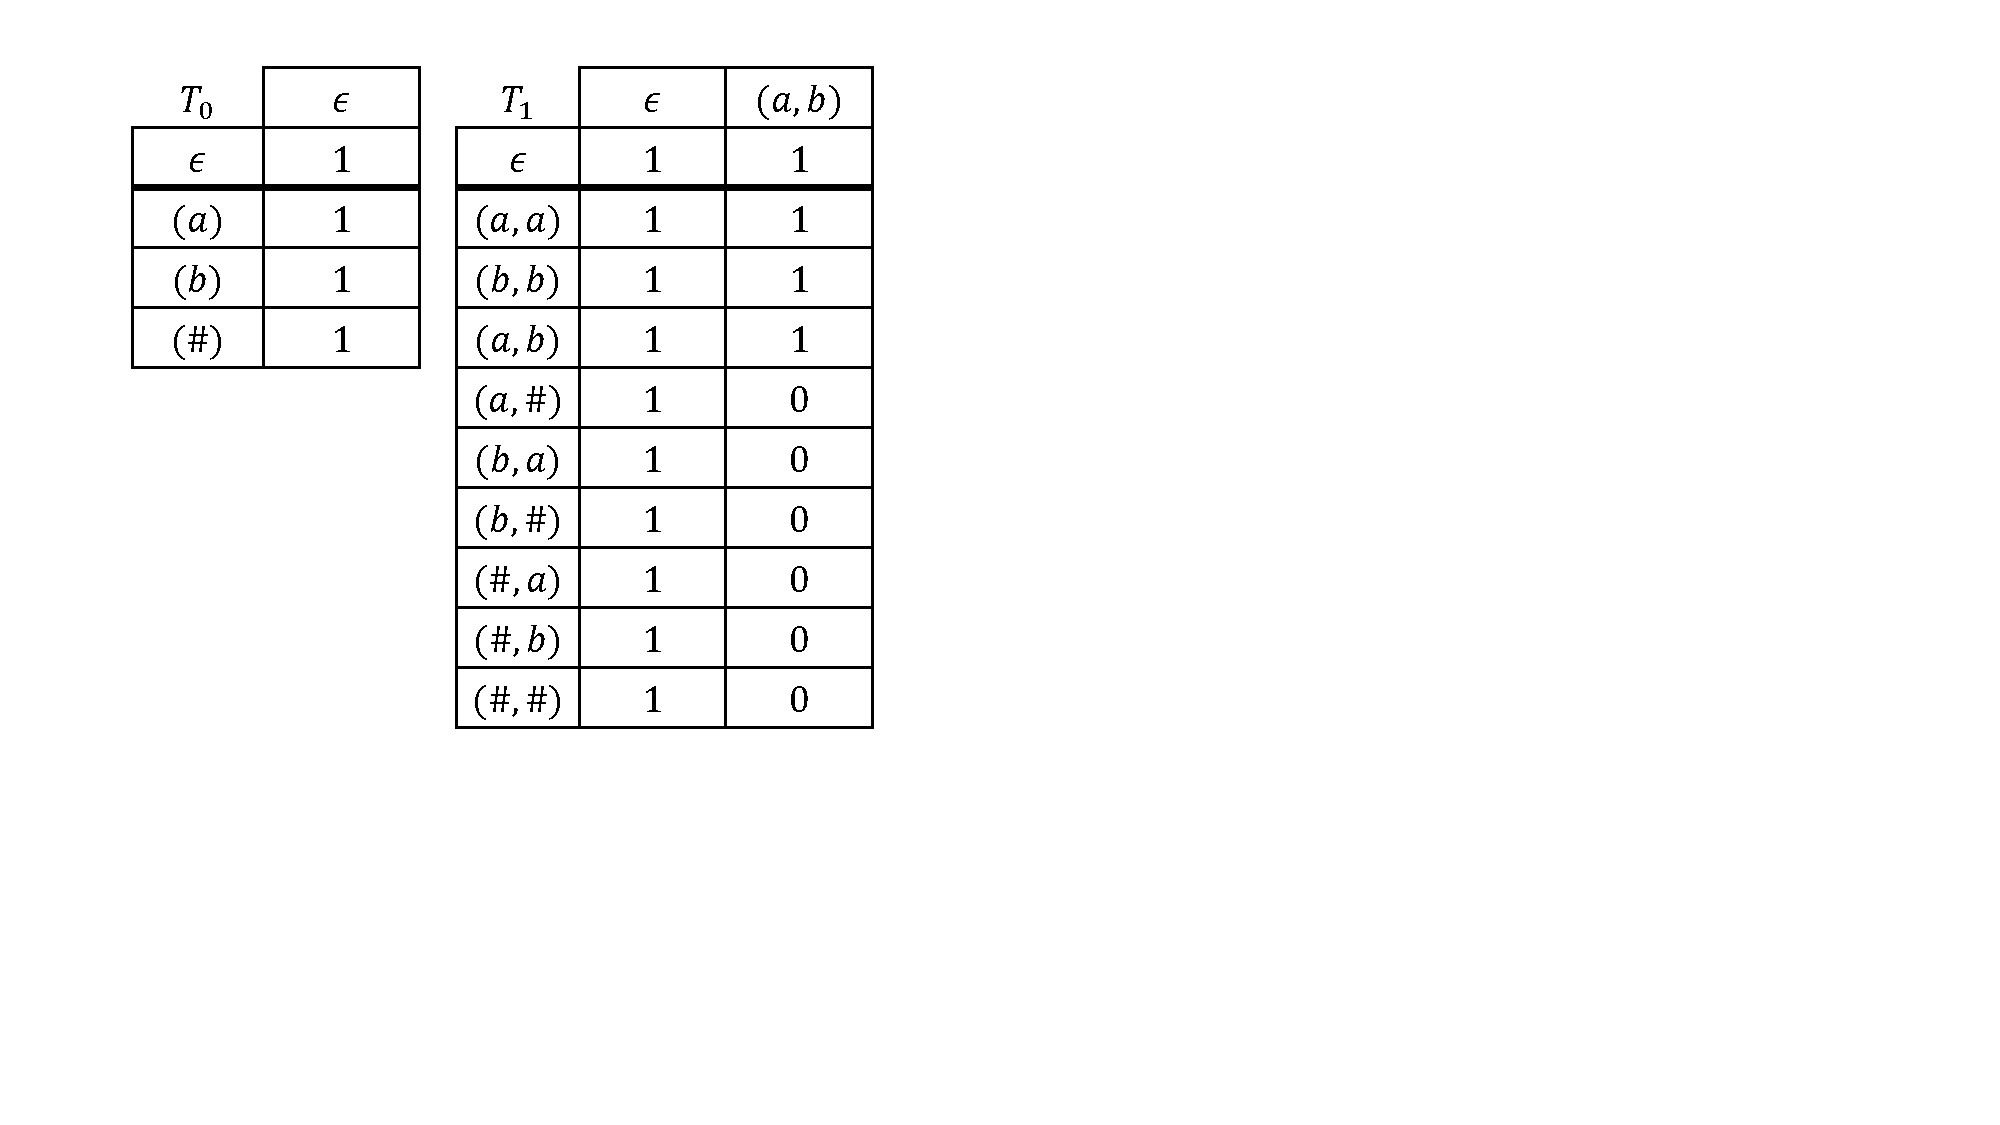
\includegraphics[scale=0.5]{figures/learning_nfhf.pdf}
    \end{center}
    \caption{The first stages of learning $\lang{\A_3}$ of Figure~\ref{fig:nfh_examples}.}
    \label{fig:learning_nfhf}
%    \hrulefill
\end{figure}

\begin{example}
Figure~\ref{fig:learning_nfhf} displays the first two stages of learning $\hlang{\A_3}$ of Figure~\ref{fig:nfh_examples}.
$T_0$ displays the initial table, with $D=E = \{\epsilon\}$, and $\hat\Sigma = \{a,b,\#\}$. since $\{a\}, \{b\}$, and $\{\epsilon\}$ are all in $\hlang{\A_3}$, the initial NFH $\A$ that the learner constructs is over a single variable, and includes, according to the answers from the membership queries, a single accepting state.

Since $\hlang{\A_3}$ includes all hyperwords of size $1$, which are now accepted by $\A$, the smallest positive counterexample the teacher can return is a hyperword of size $2$, which, in the example, is $\{a,b\}$. Table $T_1$ is then obtained from $T_0$ by applying $\uparrow_1^2$, updating the alphabet $\hat\Sigma$ to $\{a,b,\#\}^2$, and updating $D\cdot\hat\Sigma$ accordingly. The table is filled by submitting membership queries. For example, for $(b,a)\in D\cdot\hat\Sigma$ and $(a,b)\in E$, the learner submits a membership query for $\{ba, ab\}$, for which the teacher returns ``no''.
\end{example}

\subsubsection{Learning $\nfhe$}

The learning process for $\nfhe$ is almost similar to the one for $\nfhf$. We briefly describe the differences. 


As in $\nfhf$, relying on the minimality of the counterexamples returned by the teacher guarantees that when a counterexample $S$ such that $|S|>k$ is returned, it is a positive counterexample. 
Indeed, assume by way of contradiction that $S$ is a negative counterexample of size $k'$. Since $\hat\A$ accepts $S$, there exists a word $\zip(w_1,\ldots w_k)$ in $\lang{\hat\A}$ such that $\{w_1,\ldots w_k\}\in S$. According to the semantics of $\exists$, if $\zip(w_1,w_2,\ldots w_k)$ in $\lang{\hat\A}$ then $S\in\hlang\A$. Since $S\notin\hl$, we have that $\{w_1,\ldots w_k\}$ is a smaller counterexample, a contradiction. 

Therefore, when the teacher returns a counterexample $S$ of size $k'>k$, the alphabet $\hat\Sigma$ is extended to $(\Sigma\cup\{\#\})^{k'}$, and the table $T$ is updated by $\uparrow_{k}^{k'}$, as is done for $\nfhf$.

If $|S|\leq k$, then $S$ may be either positive or negative. If $S$ is negative, then there exists some permutation $w$ of $S$ that is accepted by $\hat\A$. However, no such permutation is in $T$, as a membership query would have returned ``no''. Similarly, if $S$ is positive, then there exists no permutation of $S$ that $\hat\A$ accepts. In both cases, the learner chooses a permutation of $S$ and adds it, along with its suffixes, to $E$. 

As in the case of $\nfhf$, the success of an equivalence query does not necessarily imply that $\A$ is permutation-complete. 
If $\A$ is not permutation-complete, the learner finds two words $w,w'$ such that $w\in\lang{\hat\A}$ but $w'\notin\lang{\hat\A}$, and adds $w'$ as a counterexample to $E$. It holds that $w'$ was not in $T$ prior to this addition.
The procedure then returns to the learning loop.



\bibliographystyle{plainurl}
\bibliography{bibliography,extra_bib}

\end{document}

